\documentclass[referee,pdflatex,sn-mathphys-num]{sn-jnl}

\usepackage{graphicx}
\usepackage{multirow}
\usepackage{amsmath,amssymb,amsfonts}
\usepackage{amsthm}
\usepackage{mathrsfs}
\usepackage[title]{appendix}
\usepackage{xcolor}
\usepackage{textcomp}
\usepackage{manyfoot}
\usepackage{booktabs}
\usepackage{algorithm}
\usepackage{algorithmicx}
\usepackage{algpseudocode}
\usepackage{listings}

% Set graphics path to the master images folder
\graphicspath{{../images/}}

%%% ADDITIONAL PACKAGES %%%

% etoolbox to get rid of underfull hbox warnings in bibliography
\usepackage{etoolbox}
\apptocmd{\sloppy}{\hbadness 10000\relax}{}{}

% anyfontsize gets rid of a warning in the logfile
\usepackage{anyfontsize}

% siunitx makes it easier to typeset units
\usepackage{siunitx}
\newcommand{\h}{\unit{\hour}}
\newcommand{\ph}{\unit{\per\hour}}
\newcommand{\um}{\unit{\micro\metre}}
\newcommand{\pums}{\unit{\per\micro\metre\squared}}
\newcommand{\nm}{\unit{\nano\mole\per\litre}}

\raggedbottom

\begin{document}

\title[Article Title]{A Computational Model Reveals the Effects of the CLASP Protein on Root Zonation in \emph{A. thaliana}}

\author*[1,2]{\fnm{First} \sur{Author}}\email{iauthor@gmail.com}

\author[2,3]{\fnm{Second} \sur{Author}}\email{iiauthor@gmail.com}
\equalcont{These authors contributed equally to this work.}

\author[1,2]{\fnm{Third} \sur{Author}}\email{iiiauthor@gmail.com}
\equalcont{These authors contributed equally to this work.}

\affil*[1]{\orgdiv{Department}, \orgname{Organization}, \orgaddress{\street{Street}, \city{City}, \postcode{100190}, \state{State}, \country{Country}}}

\affil[2]{\orgdiv{Department}, \orgname{Organization}, \orgaddress{\street{Street}, \city{City}, \postcode{10587}, \state{State}, \country{Country}}}

\affil[3]{\orgdiv{Department}, \orgname{Organization}, \orgaddress{\street{Street}, \city{City}, \postcode{610101}, \state{State}, \country{Country}}}

\abstract{Variations in the rates of cell division and elongation in the root apical meristem of \emph{A. thaliana} have a significant influence on organ development. In particular, the plant hormone brassinosteroid promotes cell elongation while the CLASP protein affects cell division by modulating the arrangement of microtubule polymers on the cell membrane. However, the precise effect of CLASP on cell-scale development remains unknown. In this paper, we develop a computational model to investigate root zonation in \emph{A. thaliana} mutants where the brassinosteroid/CLASP signalling network has been perturbed. The model is based on brassinosteroid receptor dynamics and their downstream effects on CLASP, cell division, and cell elongation. Fitting the model to experimental data reveals that both superphysiological and supraphysiological concentrations of CLASP inhibit cell division. These findings suggest that the efficient relocalization of microtubules between phases of the cell cycle requires the CLASP protein to be well-regulated.}

\keywords{Brassinosteroid, Cell Division, CLASP, Microtubules, Root Zonation}

\maketitle

\section{Introduction}\label{sec1}

Environmental stressors such as drought, heat, and cold have been shown to drive significant changes in the hormone and protein levels of plants \cite{halat2020}. As a result of these fluctuations, plants often undergo profound changes in development. Developing a better understanding of how hormones and proteins interact to drive tissue-scale behaviour is essential for the increasingly important field of sustainable agriculture. One system of interest for this phenomenon is the root apical meristem of \emph{A. thaliana}, where the transition from cell division to elongation is tightly regulated by multiple hormones and proteins. In this paper, we present a novel model of root zonation in the meristem based on a signalling network involving brassinosteroid (BR) and the Cytoplasmic Linker Associated Protein (CLASP).

Cell elongation is driven by turgor pressure, the force exerted by intracellular fluid on the plasma membrane. The organized deposition of cellulose microfibrils on the cell wall creates anisotropic resistance to the uniform turgor pressure, causing the unidirectional growth observed in the meristem \cite{hamant2010}. The arrangement of tubulin polymers known as microtubules has been shown to guide cellulose deposition on the cell wall \cite{hamant2010}. However, it is not known if this effect is significant enough to drive changes in cell elongation. The CLASP protein plays an essential role in microtubule patterning by helping microtubules cross sharp edges on the cell membrane \cite{ambrose2011}. This results in the formation of bundles of microtubules along the transverse and radial edges of the cell known as transfacial bundles (TFBs) \cite{halat2022}. TFBs are only observed in mitotic cells \cite{ambrose2011}, although it remains unknown whether this relationship is causal \cite{halat2022}. 

Brassinosteroids are a class of plant hormones that have been shown to promote cell growth \cite{ackerman-lavert2020}. Extracellular BRs, particularly the highly potent brassinolide (BL), bind to the BR receptor BRI1 and its homologues on the cell membrane \cite{vukasinovic2021}. Bound BRI1 receptors release the inhibition of the BZR1/BES1 transcription factors by the BIN2 signalling inhibitor \cite{ackerman-lavert2020}. BR signalling levels reach a maximum in the proximal region of the meristem due to a high concentration of BR precursors \cite{vukasinovic2021}, which drives rapid cell elongation. The BZR1/BES1 transcription factors, often used as a proxy for BR signalling, have been shown to inhibit CLASP by binding directly to its promoter and repressing its activity \cite{ruan2018}. Additionally, CLASP influences BR signalling by promoting the recycling of endocytosed BRI1 receptors \cite{ruan2018}. Together, these two effects produce a positive-negative feedback loop that helps to maintain homeostasis in the root \cite{ruan2018}.

Making small changes to the BR/CLASP signalling network leads to significant changes in root phenotypes. This paper explores the \emph{clasp-1} \cite{ambrose2007} and \emph{brinCLASPpro} \cite{ruan2018} mutant roots. The \emph{clasp-1} root has a loss-of-function mutation that fully inhibits the production of CLASP. This causes microtubules to form organized transverse arrays (OTAs) and induces premature exit from the cell cycle \cite{halat2022}. Images of the \emph{clasp-1} root reveal longer cells and a shorter organ relative to the wild type. The \emph{brinCLASPpro} root is insensitive to the effects of BR signalling, which releases the inhibition of the CLASP promoter. The resulting excess of CLASP promotes the recycling of endocytosed BRI1 receptors \cite{ruan2018}, which leads to higher concentrations of the BZR1/BES1 transcription factor. Higher levels of BR signalling induce rapid cell elongation, which causes the \emph{brinCLASPpro} root to develop longer cells relative to the wild type. However, these cells are shorter than those observed in the \emph{clasp-1} mutant. Additionally, organ size in the \emph{brinCLASPpro} root is smaller than in the wild type but larger than in the \emph{clasp-1} mutant.

In this paper, we study the signalling network shown in Figure \ref{network} using a system of time-dependent ordinary differential equations (ODEs). By fitting the numerical solutions to these equations to experimental data, we show that our current understanding of the BR/CLASP signalling network cannot differentiate the wild type root from the \emph{brinCLASPpro} mutant. Then, we investigate two biologically motivated adjustments to the model for recovering the \emph{brinCLASPpro} mutant. Ultimately, we find strong evidence that the CLASP protein inhibits cell division at superphysiological concentrations. We speculate on the biological mechanisms that drive this phenomenon and suggest avenues for further \emph{in-vivo} and \emph{in-silico} research.

\begin{figure}
\centering
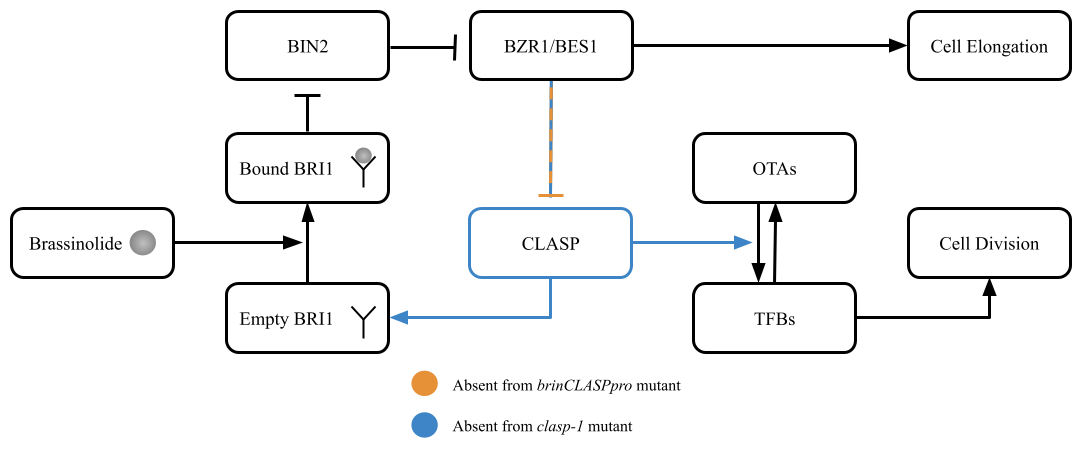
\includegraphics[width=\textwidth]{network-complete.png}
\caption{Known effects of BR and CLASP signalling on cell elongation and division in the meristem of \emph{A. thaliana}. Pointed arrows denote promotion, while flat arrows denote inhibition. Components of the signalling network that are removed in the \emph{brinCLASPpro} and \emph{clasp-1} mutants are indicated in orange and blue respectively. Exogenous BL molecules bind to empty BRI1 receptors to create bound BRI1 receptors, which release the inhibition of the BES1 transcription factor. The BES1 transcription factor inhibits the CLASP promoter and promotes cell elongation. The CLASP protein promotes the recycling of endocytosed BRI1 receptors and induces the formation of TFBs over sharp edges on the cell membrane. TFBs are closely linked with cell division, although the exact mechanism by which they are connected remains unknown. }
\label{network}
\end{figure}

\section{Methods}\label{sec11}

\subsection{Data}

Data for the model was collected from cells in the epidermal columns of \emph{in-vivo} roots and transformed into units of position and length. Data collected from trichoblast cells was used for model fitting, as shown in Figure \ref{data-binned}. For more information about the procedures used to collect and process the data, as well as some additional figures, see Appendix \ref{secA1}. The model was also fitted to data from atrichoblast cells. The results of this experiment are presented in Appendix \ref{secA4}.

\begin{figure}
\centering
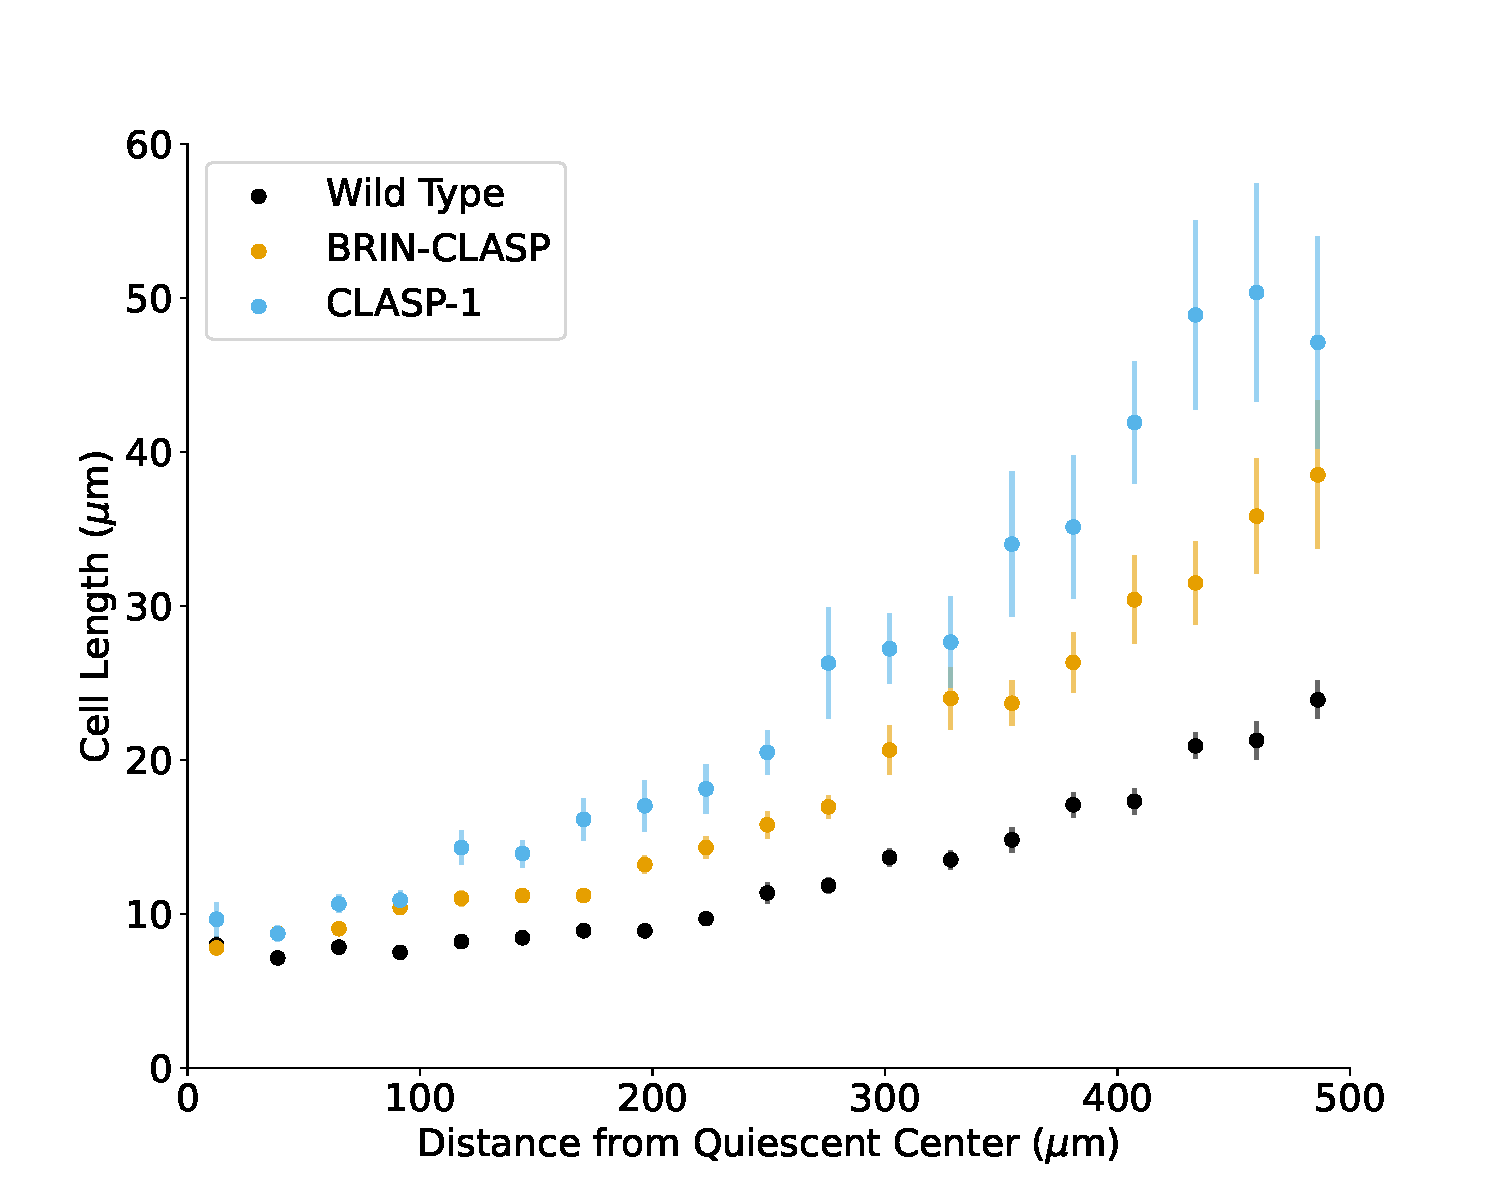
\includegraphics[width=\textwidth]{data-binned-500.pdf}
\caption{Mean cell lengths in the root apical meristem by position. The plotted points represent the mean cell length for cells of each mutant within a $25\um$ bin. Error bars denote the standard error of the mean $\hat{\sigma}_{x}^{-} = \sigma_{x} / \sqrt{n}$, where $\sigma_{x}$ denotes the sample standard deviation and $n$ denotes the number of samples in the bin. The cells of the \emph{clasp-1} mutant are the largest in all positions shown, followed by the \emph{brinCLASPpro} mutant and the wild type. These differences are statistically significant.}
\label{data-binned}
\end{figure}

\subsection{Mathematical Modelling}\label{22}

We begin by defining a model of the BRI1 receptor system using the mass balance equations \eqref{eq} presented by van Esse et al., 2012 \cite{vanesse2012}. Let $R_{T}$, $R_{F}$, and $R_{B}$ denote the concentrations of total BRI1 receptors, free BRI1 receptors, and bound BRI1 receptors respectively. Let $B(p)$ denote the extracellular BL concentration as an increasing function of cell position. Additionally, let $B_{F}$ and $B_{B}$ denote the concentration of free and bound BL ligand respectively. Let $K_{d}$ be the rate at which BL molecules dissociate from BRI1 receptors.

\begin{equation}
\begin{cases}
    \label{eq}
    R_{B} = \dfrac{R_{F} \cdot B_{F}}{K_{d}} \\
    R_{T} = R_{B} + R_{F} \\
    B = B_{B} + B_{F} 
\end{cases}
\end{equation}

By rearranging Equation \eqref{eq}, we can solve for $R_{B}$ as a function of $R_{T}$ and $B$ \eqref{bri1}. Note that Equation \eqref{bri1} is implicitly a function of position because extracellular BL concentration depends on cell position in the meristem.

\begin{equation}
\label{bri1}
R_{B} = \frac{(B + R_{T} + K_{d}) - \sqrt{(B + R_{T} + K_{d})^{2} - 4 \cdot  R_{T} \cdot B}}{2}
\end{equation}

The literature contains estimates for $R_{T}$ and $K_{d}$. van Esse et al., 2012 \cite{vanesse2012} estimate the BRI1 receptor concentration to be $62 \pm 4 \nm$ in wild type roots. Estimates of the BL dissociation constant $K_{d}$ range from $7.4 \nm$ to $15 \nm$ \cite{wang2001} up to $55 \nm$ \cite{cano-delgado2004}. Additionally, the scale of $B$ is estimated to be no larger than $1\nm$ \cite{vanesse2012}. Our model assumes that all BRI1 receptors are localized to the cell membrane. Additionally, we assume that the law of mass action is a reasonable approximation for the diffusing BL ligand binding to the static BRI1 receptors. We believe this decision is justified due to the low occupancy of the BRI1 receptors \cite{vanesse2012}, which suggests that any free BL ligand will have many opportunities to bind to a receptor. Further modelling of the BRI1 receptor network using a more detailed approach would help to clarify and refine these assumptions.

Using the $R_{B}$ function in Equation \eqref{bri1}, we derive a mathematical description of the intracellular dynamics of the BR/CLASP signalling network \eqref{intracellular-final}. These equations are derived from a system of ODEs under a quasi-steady state (QSS) assumption. In other words, we assume that intracellular processes such as receptor binding, the inhibition of the CLASP promoter, and the transcription of BES1 occur at a much faster time scale than cell division and elongation. Since $\text{BES1}$ becomes a scalar multiple of $R_{B}$ under the QSS assumption, $R_{B}$ will be used in place of $\text{BES1}$ in the model. The CLASP concentration $C$ is non-dimensionalized such that $C = 1$ corresponds to the average CLASP level in the wild type. The total receptor concentration $R_{T}$ in the \emph{clasp-1} mutant is $65\%$ of the wild type concentration based on experimental observations \cite{ruan2018}. For the original set of ODEs and details about how these equations were transformed, see Appendix \ref{secA2}.

\begin{equation}
\label{intracellular-final}
\begin{aligned}
  C &= \beta_{0} - \beta_{1}R_{B} \\[5pt]
  R_{T} &= 62 (0.65 + 0.35 C)
\end{aligned}
\end{equation}

The intracellular dynamics influence the rates of cell division and elongation through the level of BES1 signalling (now represented by $R_{B}$) and the concentration of the CLASP protein. We include cell division and elongation in our model by adding the two differential equations presented in Equation \eqref{extracellular-final}. In these equations, cells grow at a basal rate $\gamma_{0}$ which is increased by BES1 at a rate $\gamma_{1}$. The rate of cell elongation is assumed to be proportional to length because longer cells have more vertical surface area for the cellulose microfibrils to stretch, tear, and reform. This modelling assumption is known in the literature, particularly Lockhart, 1965 \cite{lockhart1965}. Cells stop growing at a length of $100\um$ based on the sizer model developed by Pavelescu et al., 2016 \cite{pavelescu2016}. The variable $D \in [0, 1]$ denotes the cell's position in the cell cycle. When $D = 1$, the cell divides into two cells of equal length with $D = 0$. Progress in the cell cycle proceeds at a basal rate of $1$, which is increased by CLASP at a rate $\delta_{0}$. We also assume that a sizer model drives the inhibition of cell division for longer cells. Through this mechanis, cell division stops completely when $L^{n} \gg \delta_{1}^{n}$. The precise details of how these equations were derived can be found in Appendix \ref{secA2}.

\begin{equation}
\label{extracellular-final}
\begin{aligned}
  \frac{ dL }{ dt } &= \left(\gamma_{0} + \gamma_{1}\text{BES1}\right)L  \\[5pt]
\frac{ dD }{ dt } &= (1 + \delta_{0}C)\left( 1 - \frac{ L^{ n } }{ \delta_{1}^{ n } + L^{ n } } \right) 
\end{aligned}
\end{equation}

\section{Results}\label{sec2}

\subsection{BES1 Signalling}\label{sec21}

We used data from Vukašinović et al. \cite{vukasinovic2021}, to fit the intracellular CLASP and BRI1 receptor equations shown in \eqref{bri1} and \eqref{intracellular-final}. The functional form of the extracellular BL function $B(p)$ is unknown, although we know the scale to be less than $1\nm$  \cite{vanesse2012}. To identify the BL function that produced the best fit to the data, we tested three candidate equations \eqref{bl-candidates}.

\begin{equation}
\label{bl-candidates}
\begin{aligned}
  \text{Linear}&: B(p) = \alpha_{0} + \frac{(1 - \alpha_{0})p}{1000} \\[5pt]
  \text{Quadratic}&: B(p) = \alpha_{0} + \frac{(1 - \alpha_{0})p^{2}}{1000^{2}} \\[5pt]
  \text{Hill}&: B(p) = \alpha_{0} + \frac{(1 - \alpha_{0})p^{2}}{\alpha_{1}^{2} + p^{2}}
\end{aligned}
\end{equation}

Since the hill function has one additional degree of freedom through the parameter $\alpha_{1}$, we used the Akaike Information Criterion (AIC) \cite{akaike1974} to account for overfitting. In particular, we use the AICc correction \cite{sugiura1978} to accommodate the small ratio between the sample size and the number of parameters. The intracellular equations in \eqref{bri1} and \eqref{intracellular-final} were solved using the computer algebra system \href{https://www.sympy.org/en/index.html}{sympy} and the optimal parameter values were identified using the DIviding RECTangles (DIRECT) global optimization algorithm \cite{jones1993} from the scientific computing package \href{https://docs.scipy.org/doc/scipy/reference/generated/scipy.optimize.direct.html}{scipy}. A total of three parameters were fitted for the QSS equations in addition to either one or two parameters for the $B(p)$ function. The fitted models are shown in Figure \ref{bl-functions}. Table \ref{bl-fits} contains information about each model including the optimal parameters, RMSE, and AICc.

\begin{figure}
  \centering
  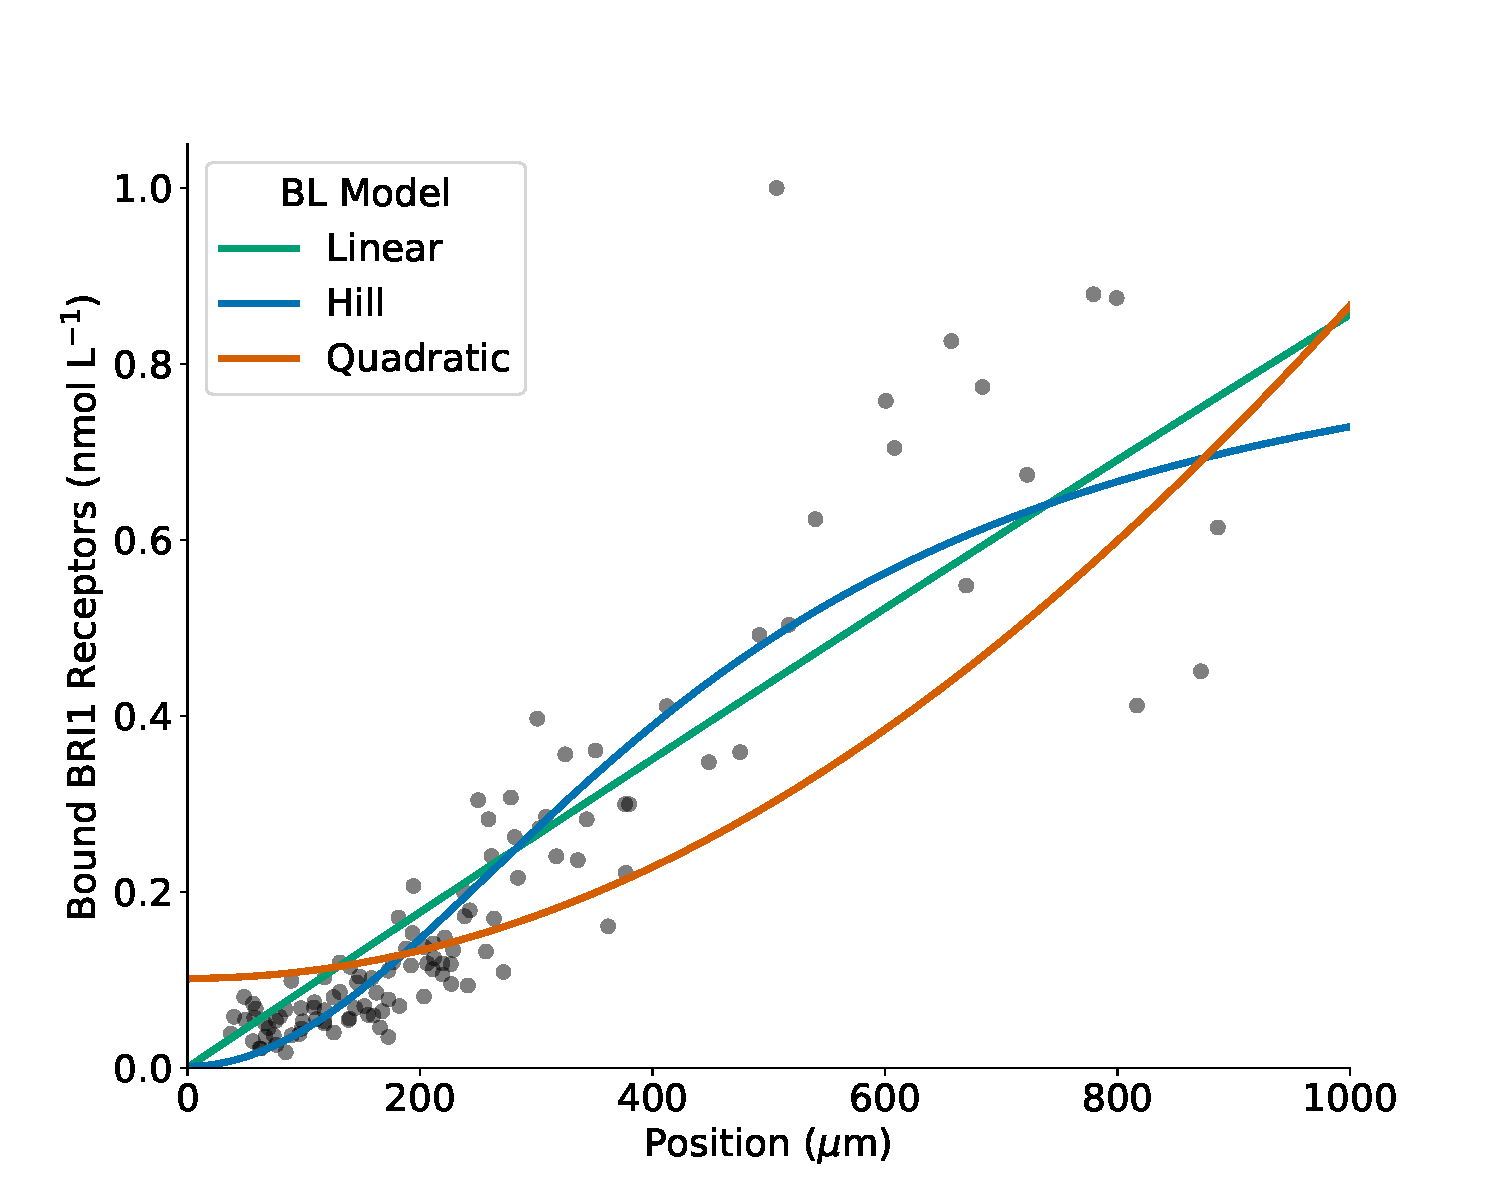
\includegraphics[width=\textwidth]{bes1-functions.pdf}
  \caption{Results of fitting the QSS equations for the CLASP protein and BRI1 receptor to experimental data \cite{vukasinovic2021}. The hill function had the lowest root-mean-squared error (RMSE) from the experimental data at $0.0889$. The linear BL function performed the next best at $0.1000$, followed by the quadratic function of $0.1296$. Further analysis is needed to determine the model with the lowest information criterion. }
  \label{bl-functions}
\end{figure}

\begin{table}[ht]
\caption{Details from the linear, hill, and quadratic models of BL. The hill function had the lowest absolute error and the highest AICc value, which suggests it may be overfitted. The low variance in the fitted values of the $\beta_{0}$, $\beta_{1}$, and $K_{d}$ parameters between models suggest that our model is robust to changes in the brassinolide function. }
\label{bl-fits}
\begin{tabular}{@{}llllllll@{}}
\toprule
BL Model & RMSE & AICc & $\alpha_{0}$ & $\alpha_{1}$ & $\beta_{0}$ & $\beta_{1}$ & $K_{d}$ \\
\midrule
Linear & $0.1000$ & $11.694$ & $0.001$ & - & $1.389$ & $0.895$ & $8.901$ \\
Hill & $0.0889$ & $13.685$ & $0.002$ & $456.104$ & $1.389$ & $0.916$ & $7.533$ \\
Quadratic & $0.1296$ & $12.470$ & $0.113$ & - & $1.389$ & $1.08$ & $7.598$ \\
\botrule
\end{tabular}
\end{table}

Since the linear BL model yielded the lowest AICc, we will use it for subsequent analyses. Figure \ref{bes1-mutants} shows the predicted concentrations of CLASP and BRI1 receptors in the mutant roots under the assumption that the exogenous BL concentration remains unchanged under the \emph{clasp-1} and \emph{brinCLASPpro} mutations. This plot shows that the model accurately reflects the BR/CLASP signalling network shown in Figure \ref{network} by predicting a higher concentration of CLASP and BRI1 receptors in the \emph{brinCLASPpro} mutant and lower concentrations of BRI1 receptors in the \emph{clasp-1} mutant.

\begin{figure}
  \centering
  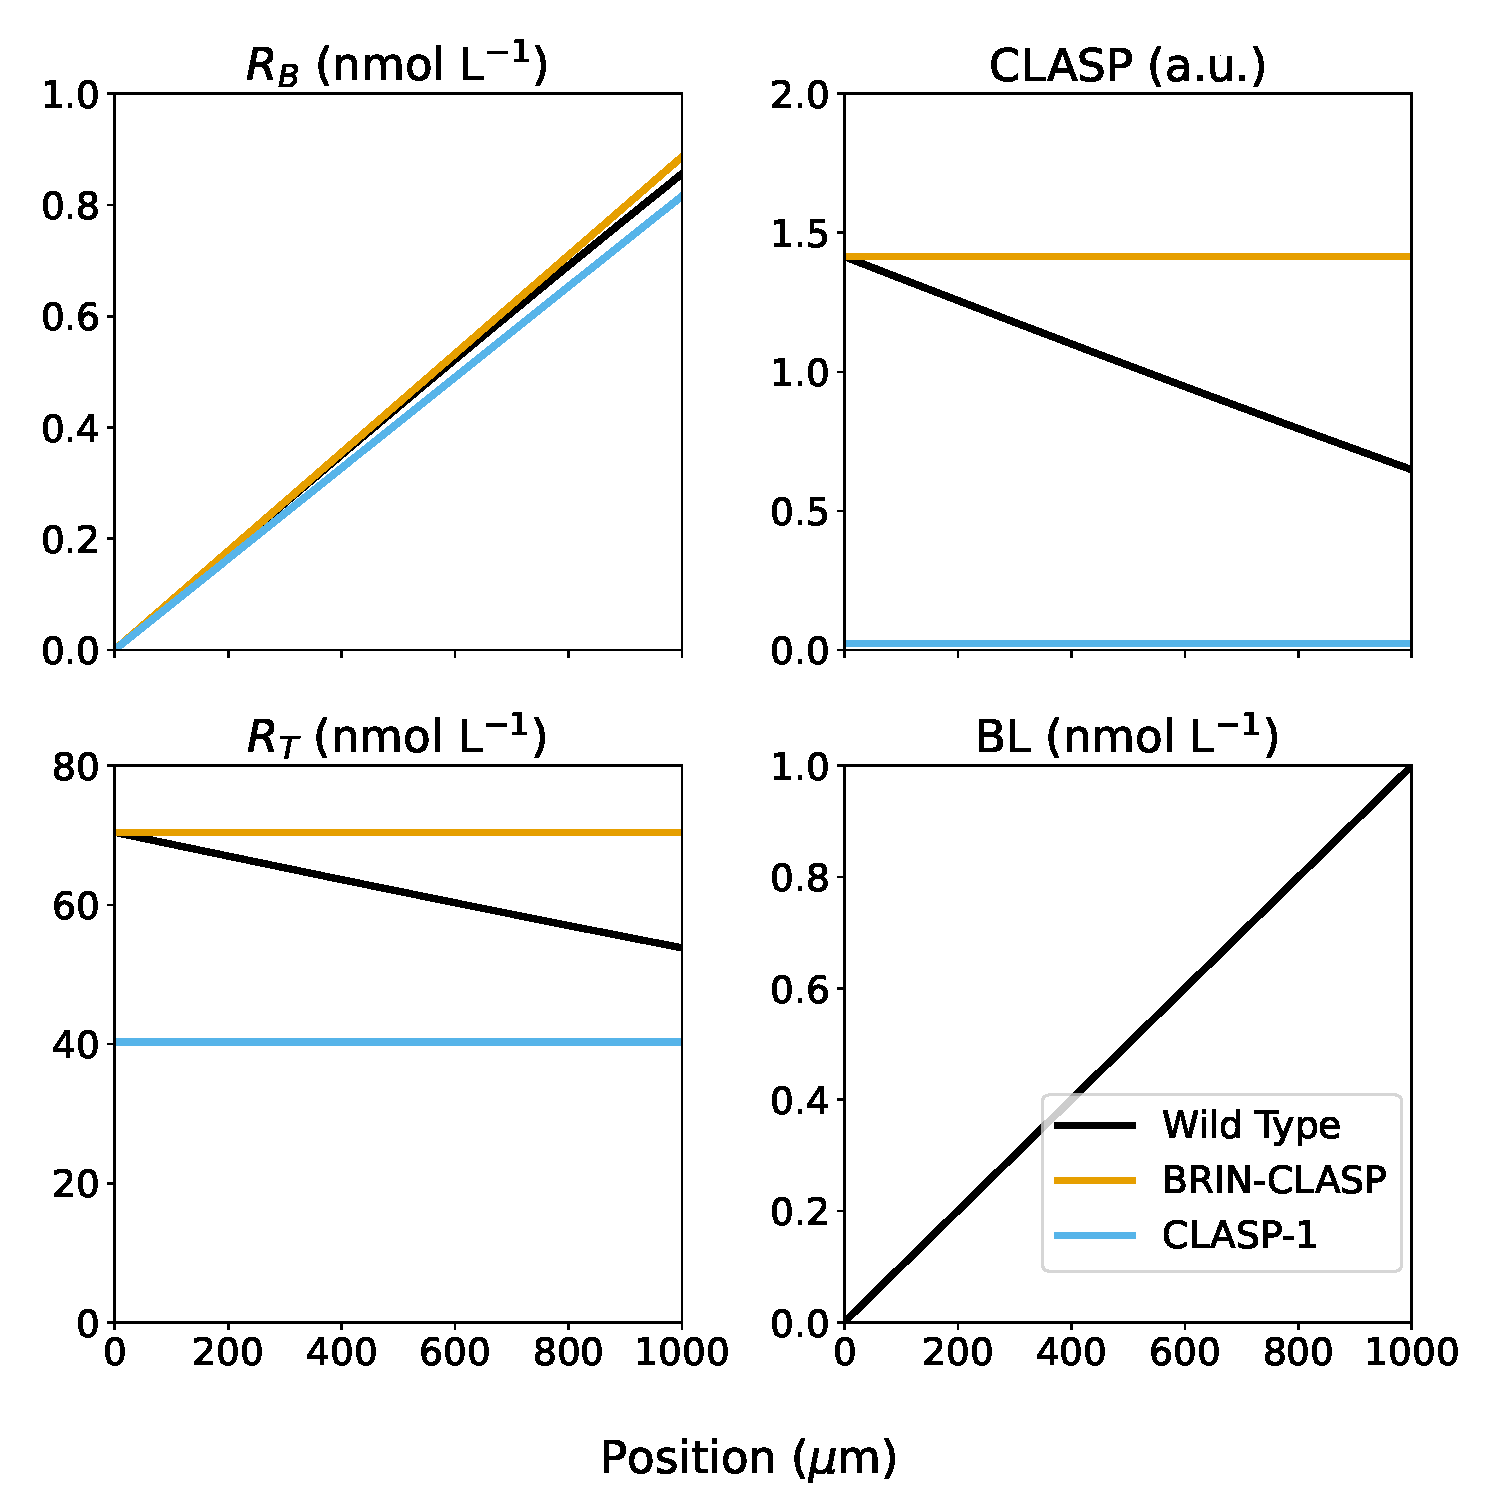
\includegraphics[width=\textwidth]{bes1-mutants.pdf}
  \caption{Results of running the fitted BES1 signalling model on the \emph{brinCLASPpro} and \emph{clasp-1} mutants using the optimal parameters shown in Table \ref{bl-fits}. The extracellular BL function is assumed to be constant across mutants. In the \emph{clasp-1} mutant, CLASP is $0$ and BRI1 receptor levels are lower than in the wild type, which reflects our current understanding of the BR/CLASP signalling network. Conversely, the \emph{brinCLASPpro} mutant exhibits higher levels of CLASP and BRI1 receptors which is also in line with the literature.}
\label{bes1-mutants}
\end{figure}

\subsection{Cell Column Modelling}

Next, we developed a model of a single column of trichoblast cells in the epidermis.  The intracellular model fitted in \ref{sec21} is used within the column model to calculate the CLASP and BRI1 concentrations. Each cell in the column model grows and divides based on Equation \eqref{extracellular-final}. An additional parameter $m$, the minimum length of a dividing cell, was added to the model to prevent the formation of unrealistically small cells. The position of each cell in the column is equal to the cumulative sum of the lengths of the cells below it. The column model was fitted to the experimental data presented in Figure \ref{data-binned} using the DIRECT algorithm \cite{jones1993}. Model accuracy was evaluated by binning cells by position and comparing the average of each bin to experimental data. The results of implementing the column model are shown in Table \ref{column-fits} and Figure \ref{column-results}.

\begin{table}[ht]
\caption{Optimal parameter values for the initial column model. $m$, the minimum length of a mitotic cell, was found to be $13.77\um$. Additionally, a $\delta_{1}$ value of $21.26\um$ indicates that a cell of this length will move through the cell cycle approximately $50\%$ slower than a short cell. }
\label{column-fits}
\begin{tabular}{@{}llllllll@{}}
\toprule
RMSE & $m$ & $\gamma_{0}$ & $\gamma_{1}$ & $\delta_{0}$ & $\delta_{1}$ \\
\midrule
$10.401$ & $13.77$ & $0.5247$ & $4.630$ & $0.2078$ & $21.26$\\
\botrule
\end{tabular}
\end{table}

\begin{figure}
  \centering
  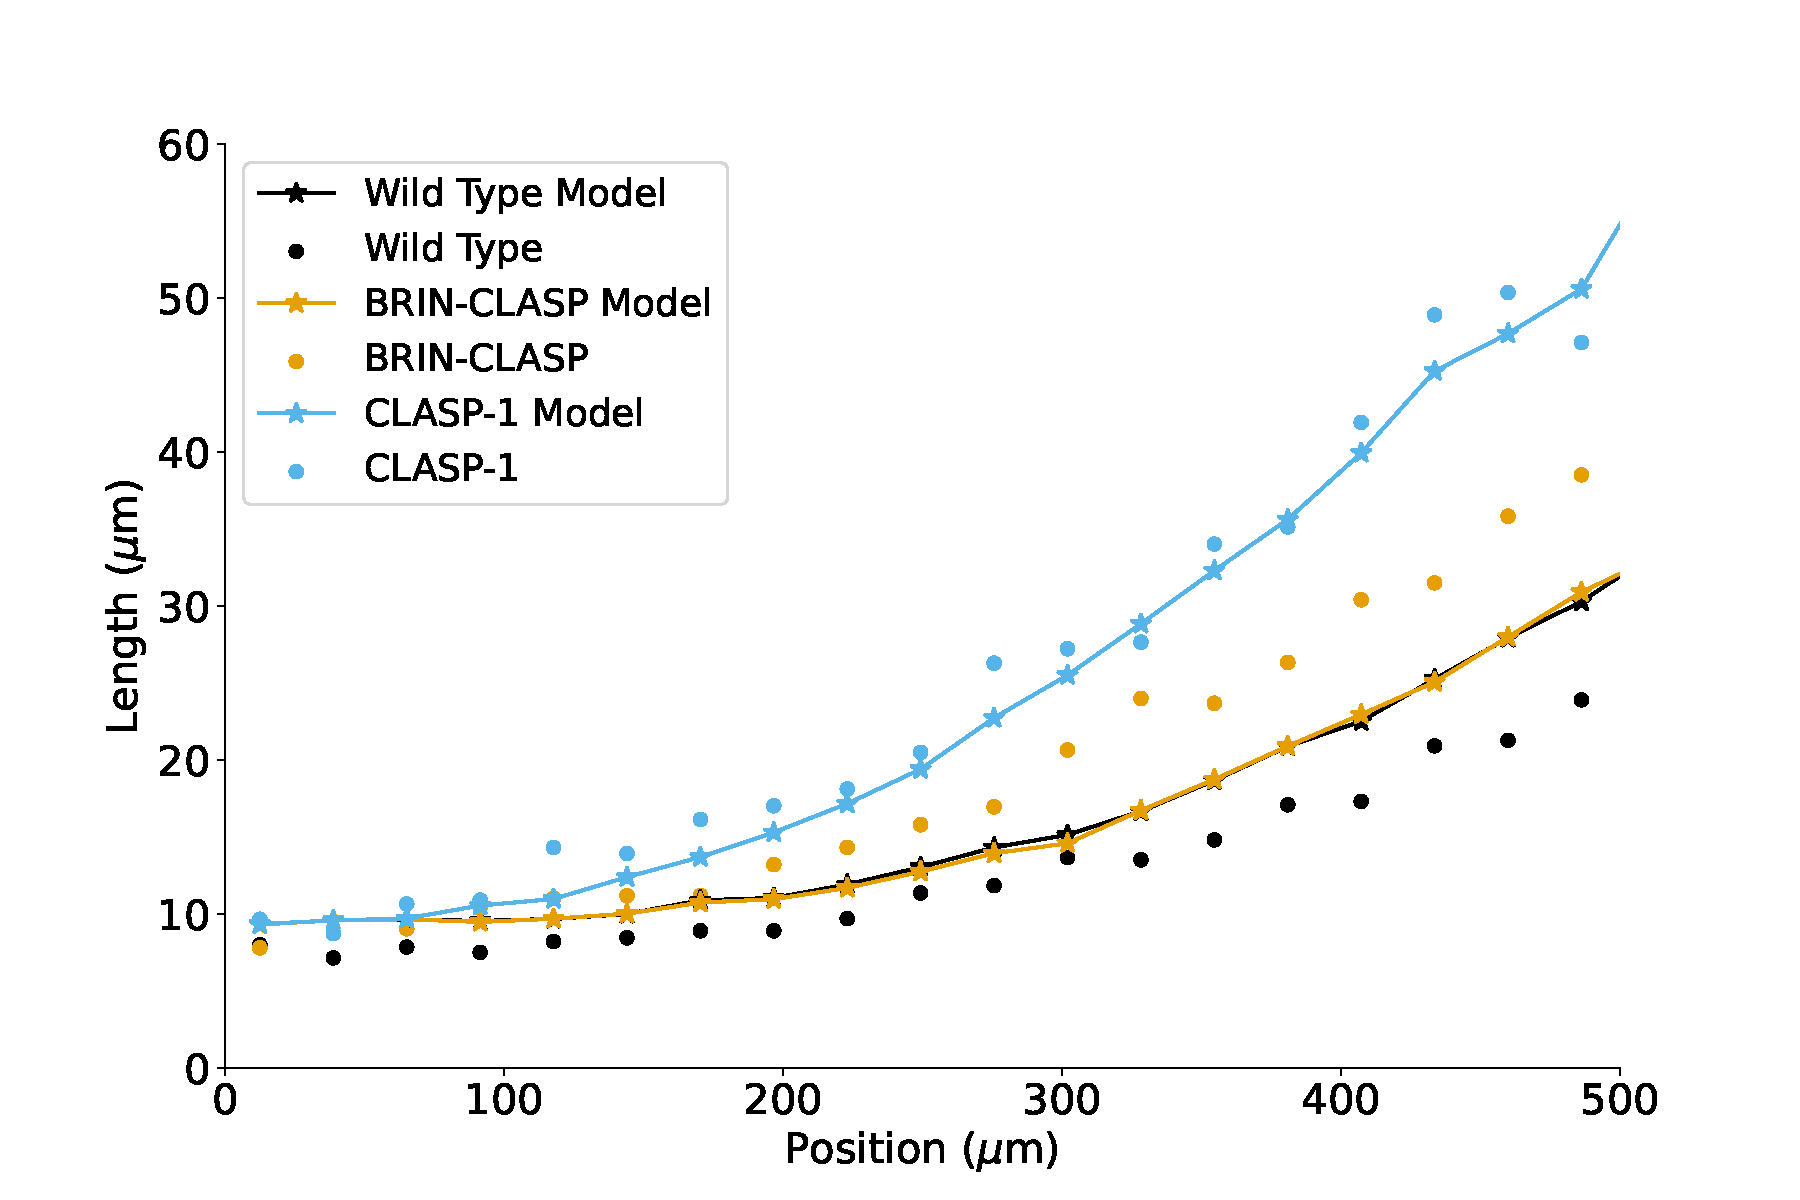
\includegraphics[width=\textwidth]{column-original-fit.pdf}
\caption{Results of fitting the column model to binned averages from experimental data. The model accurately predicted the behaviour of the \emph{clasp-1} mutant within the standard error of the mean for most positions in the root. However, the model could not differentiate between the wild type root and \emph{brinCLASPpro} mutant. This can be observed by the significant overlap between the black and orange "x" markers on the plot above. }
\label{column-results}
\end{figure}

The model struggled to differentiate between the wild type and the \emph{brinCLASPpro} mutant. This may be because the bound BRI1 receptor level $R_{B}$ is essentially the same across all three mutants as shown in Figure \ref{bes1-mutants}. This means the \emph{brinCLASPpro} mutant does not grow significantly faster than the wild type, leading to similar cell sizes. Additionally, the \emph{brinCLASPpro} mutant has a higher CLASP concentration than the wild type, especially at higher positions in the root. In theory, cells in the \emph{brinCLASPpro} root should divide more often, leading to shorter cells. However, it appears that this effect was minimized during parameter optimization. Qualitatively, there are two ways to differentiate the \emph{brinCLASPpro} mutant from the wild type: decrease its division rate or increase its growth rate. In the remainder of this paper, we discuss two potential mechanisms for differentiating the \emph{brinCLASPpro} mutant from the wild type. Then, we evaluate their validity by adjusting the intracellular and column models and fitting them to experimental data.

\subsection{Varying BRI1 Receptor Levels}

The relationship between the bound BRI1 receptors $R_{B}$ and the total BRI1 receptors $R_{T}$ is based on the mass balance equations shown in Equation \eqref{eq}. Under these equations, increasing $R_{T}$ has diminishing effects on $R_{B}$ provided that the extracellular BL level $B$ is constant. Since no more than $2\%$ of the BRI1 receptors are bound at any location in the root, the increased $R_{T}$ level in the \emph{brinCLASPpro} root has almost no effect on $R_{B}$ relative to the wild type. Therefore, modifying the ratio between $B$ and $R_{B}$ to be closer to saturation is one mechanism for differentiating the \emph{brinCLASPpro} mutant from the wild type. There are two ways to implement this change in the intracellular model: increasing $B$ and decreasing $R_{T}$. The chosen $R_{T}$ value of $62\nm$ is based on experimental observations of wild type roots \cite{vanesse2011}, so we decided to fix $R_{T}$ and increase $B$ instead. There is a biological justification for this change. Although BL is the most biochemically active brassinosteroid in the meristem, other brassinosteroids are also present \cite{vukasinovic2021, ackerman-lavert2020}. The new value $B^{*} = \omega B$ where $\omega > 1$ can be interpreted as the bound BRI1 receptor level accounting for the presence of other brassinosteroids. 

Implementing the modification outlined above uncovered a system-scale issue with attempting to modify the ratio between $R_{T}$ and $B$ to increase the rate of growth in the \emph{brinCLASPpro} mutant. The BES1 concentrations shown in Figure \ref{bl-functions} are approximately $5$ times higher in the proximal meristem ($600\um$ to $1000\um$) than in the distal meristem ($0\um$ to $300\um$). This means that multiplying the extracellular BL function by a scalar will produce an outsized effect on the cells located higher in the root. However, the growth rate of these cells is not relevant to the behaviour of the column model, since cells above $600\um$ are not mitotic and will grow to a final length of $100\um$ irrespective of BR signalling. This phenomenon means that the value of $\omega$ had to be increased to biologically unreasonable levels before significant changes in the BRI1 receptor system were observed in the distal meristem. For the results of these simulations, see Figure \ref{bes1-mutants-modified}. We also attempted to rescale $B$ using a linear function of the form $B^{*} = \omega_{0}B + \omega_{1}$. This equation corresponds to the biological hypothesis that some of the additional brassinosteroids are distributed uniformly across the length of the meristem. However, adjusting the BRI1 receptor system in this manner caused the most distal cells to grow too rapidly, preventing the gradual increase in cell length shown in Figure \ref{data-binned}.
 
\subsection{Modifying CLASP's Influence on Division} 

The \emph{brinCLASPpro} mutant has a higher concentration of CLASP which results in a higher rate of division under our current model. However, this phenomenon is not observed \emph{in-vivo}, leading us to believe that the relationship between CLASP and cell division may be more complicated. We speculate that CLASP stabilizes microtubule polymers until the cell is ready to move to the next phase in the cell cycle. This means that both superphysiological and supraphysiological concentrations of CLASP can inhibit cell division. If CLASP is absent as in the \emph{clasp-1} mutant, we observe a loose pre-prophase band \cite{ambrose2007} caused by the absence of microtubule rescue. This inhibits cell division by slowing down mitosis. If CLASP is high as in the \emph{brinCLASPpro} mutant, we suspect that the transfacial bundles that form in cell interphase are too rigid. Because these transfacial bundles take longer to disassemble when the cell enters mitosis, cells in the \emph{brinCLASPpro} mutant also take longer to divide relative to the wild type. To summarize, we believe that CLASP inhibits division at both sufficiently low and sufficiently high concentrations. This assumption can be represented in our model by modifying the division equation to include new parameters $\sigma_{0}$ and $\sigma_{1}$. The fitted model after this modification is shown in Figure \ref{column-modified-fit} and Table \ref{column-modified-parameters}.

\begin{equation}
\label{division-modified}
\frac{dD}{dt} = \left( \sigma_{0} + \sigma_{1}C - C^{2} \right)\left( 1 - \frac{L^{n}}{\delta_{1}^{n} + L^{n}} \right) 
\end{equation}


\begin{table}[!ht]
\centering
\caption{Optimal parameter values for the fitted column model after modifying the division function. The global maximum of the $dD/dt$ function occurs at $C^{*} = 0.732$. The minimum length of a mitotic cell was found to be $m = 11.69$. The fact that $\gamma_{1} \gg \gamma_{0}$ indicates that the majority of cell growth is driven by brassinosteroids. }
\label{column-modified-parameters}
\begin{tabular}{@{}llllllll@{}}
\toprule
RMSE & $m$ & $\gamma_{0}$ & $\gamma_{1}$ & $\delta_{1}$ & $\sigma_{0}$ & $\sigma_{1}$ \\
\midrule
$4.648$ & $11.69$ & $0.4877$ & $4.165$ & $23.44$ & $0.8333$ & $1.463$ \\
\botrule
\end{tabular}
\end{table}

\begin{figure}
  \centering
  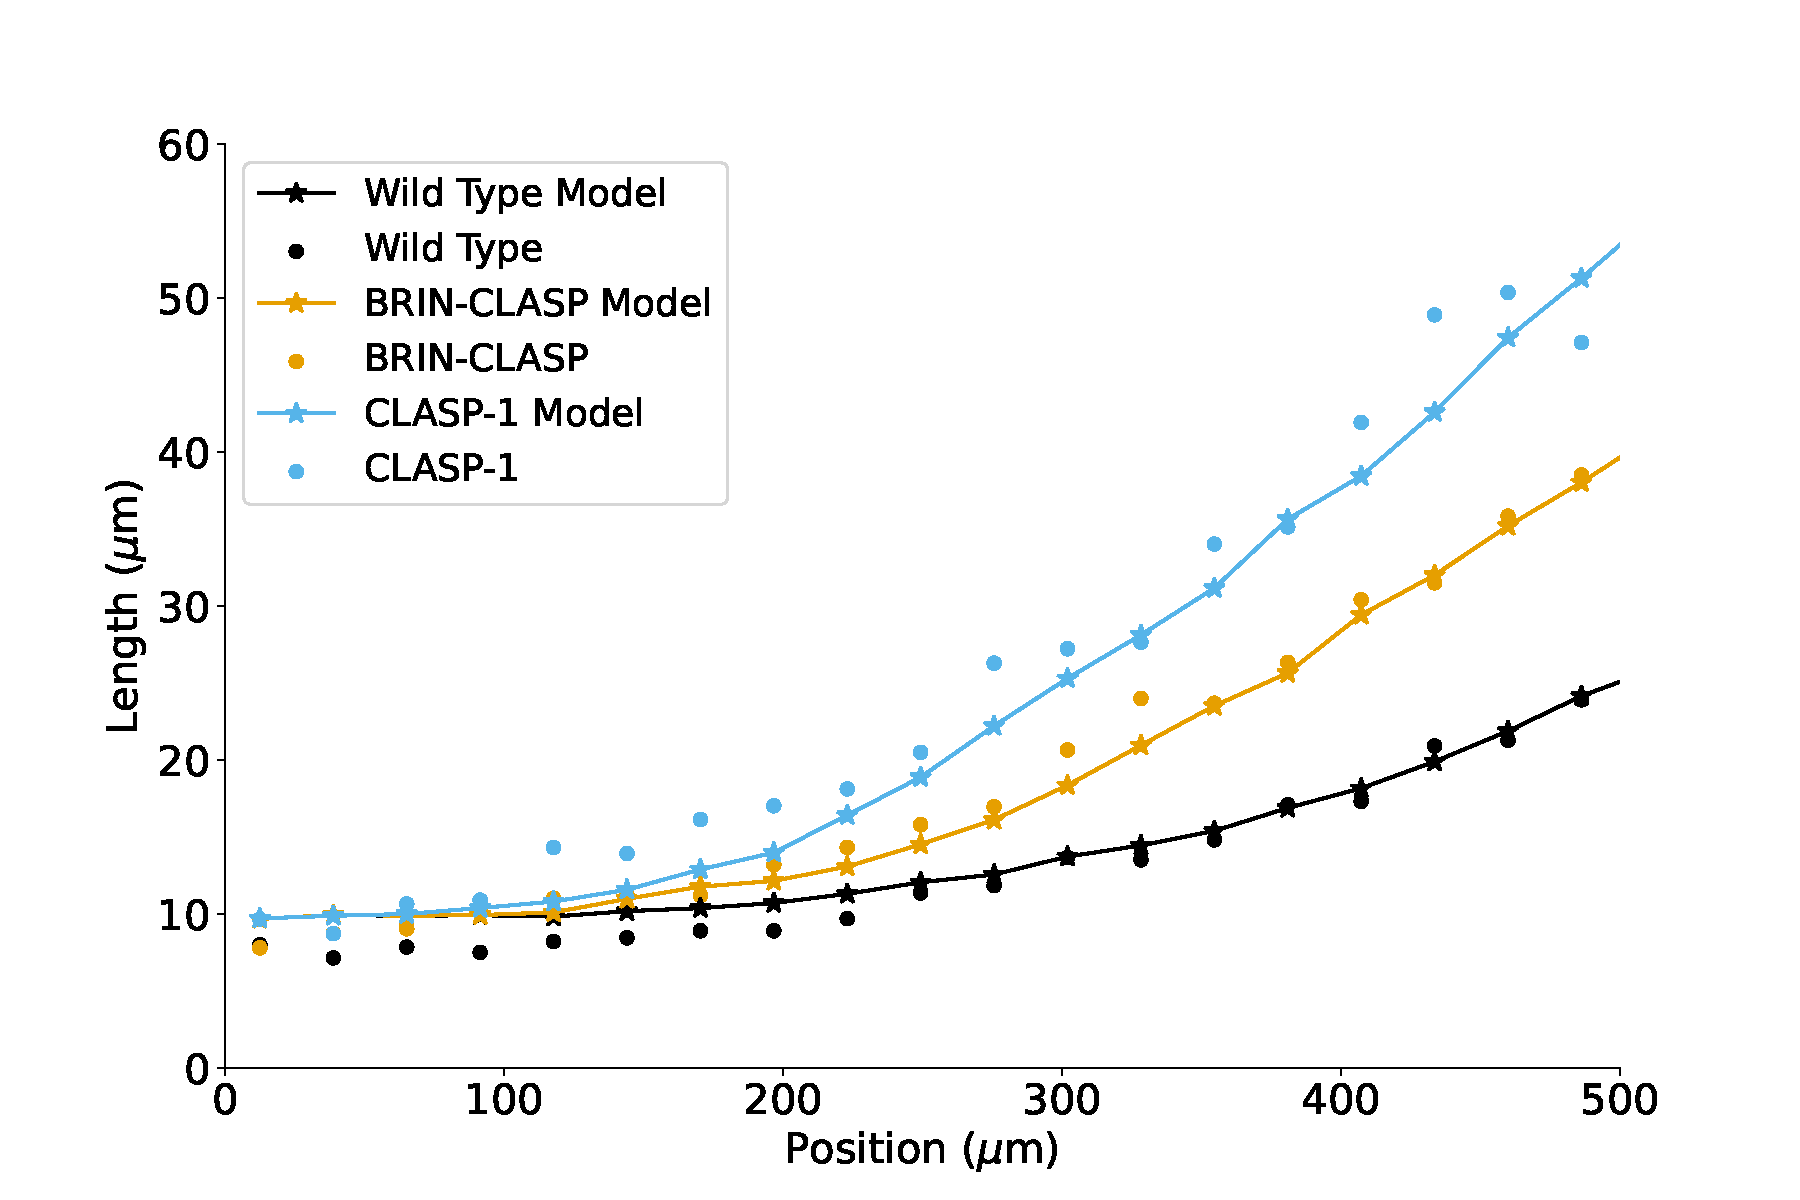
\includegraphics[width=\textwidth]{column-modified-fit.pdf}
  \caption{Model results after modifying CLASP's influence on division. By making CLASP inhibit division at high concentrations, the RMSE of the model decreased from $10.401$ to $4.648$. Under the new model, the length profiles of the wild type and \emph{brinCLASPpro} mutants are clearly differentiated. }
  \label{column-modified-fit}
\end{figure}

 
\section{Discussion}\label{sec12}

In this paper, we developed a novel ODE model of BR/CLASP signalling in the meristem of \emph{A. thaliana} roots. We built this model based on \emph{in-vivo} experiments involving the CLASP protein \cite{ambrose2011, ruan2018, halat2022} and previous models of the BRI1 receptor system \cite{vanesse2012}. Initially, our model could not differentiate the \emph{brinCLASPpro} mutant from the wild type. However, a modified model that includes the inhibition of cell division by superphysiological concentrations of CLASP was sufficient to explain the wild type and both mutants. Our hypothesis for the biological mechanism driving this behaviour is that the CLASP protein is responsible for ensuring microtubule stability during each phase of the cell cycle. Therefore, high concentrations of CLASP prevent the transfacial microtubule bundles that form during cell interphase from disassembling during mitosis, leading to a slower cell cycle. However, further experimental research is needed to explore the validity of this hypothesis.

Our model makes use of two "sizer" mechanisms, one for cell differentiation proposed by Pavelescu et al., 2016 \cite{pavelescu2016}, and a novel "sizer" mechanism for division zone exit.  When these mechanisms are modelled together, organ size is directly proportional to the number of division events, which is approximately proportional to the size of the division zone. Organ size is proportional to the number of division events because all cells eventually reach the same mature size. This means that the growth rate of individual cells has no effect on meristem size, assuming the model is in steady state. The sizer mechanism for division zone exit places an upper bound on cell lengths in the division zone. This means that the length of the division zone is approximately proportional to the number of mitotic cells in the root. In our experience, the use of a "sizer" mechanism for division zone exit produces a robust and biologically accurate model. However, further modelling research is still needed to compare the "sizer" mechanism with alternatives.
 
Multiple simplifying assumptions were made to reduce the dimensionality of the parameter space. First, the brassinolide concentration function was assumed to have a simple form. Receptor binding was assumed to occur at a ratio of one monomer to one ligand. Additionally, the entire intracellular system was assumed to be in a steady state. These assumptions could be loosened with quantitative measurements of BL and BES1 concentrations over time. The model of cell growth abstracted a complex signalling network involving wall-loosening enzymes, cellulose microfibrils, and microtubules \cite{smithers2024} into just two parameters $\gamma_{0}$ and $\gamma_{1}$. Implementing a mechanics-informed model of the cell wall would improve parameter estimation in subsequent models. Our model of cell division notably omits the stages of the cell cycle, such as the formation of the mitotic spindle. A more intricate model would give us a better understanding of how the CLASP protein affects cell division, and either verify or disprove our hypothesis about the role of CLASP.

Further modelling work in this area would benefit from "zooming in" on intracellular processes and "zooming out" to incorporate CLASP in models of other root hormones. There have been multiple efforts in recent years to simulate the formation of microtubules on the lipid membrane \cite{tian2023, tindemans2014, allard2010a}. These models have given us a better understanding of how microtubules behave in the presence of the CLASP protein. By coarse-graining the key results from these models, we can develop a better understanding of how microtubules influence both cell and organ development. There have also been multiple efforts to model the auxin signalling network \cite{grieneisen2007, dimambro2017}. These models have improved our understanding of hormone fluxes across the entire root, including between cell columns. Comprehensive models of the \emph{A. thaliana} root have included many molecules in addition to auxin, including cytokinins \cite{salvi2020}, ethylene \cite{moore2024}, and gibberelin \cite{muraro2016}. We believe that the BR signalling network and its influence on the CLASP protein should also be included in these models. Developing mathematical models of the influence of hormones and proteins on intracellular processes, cell development, and organ development remains a pressing area for further research. With a better understanding of how plants grow from the smallest scales to the largest, we can protect our crops from droughts, floods, and other adverse events while improving their yield and reproductive capacity.

\backmatter

\bmhead*{Supplementary Information}

The code for this project is available on \href{https://github.com/rileywheadon/clasp-model}{Github}.

\bmhead*{Acknowledgements}

TBD

\section*{Declarations}

TBD

\bibliography{sources}

\begin{appendices}

\section{Data Collection and Preparation}\label{secA1}

Five distinct lines of \emph{A. thaliana} were grown in the lab. Table \ref{plant-lines} contains the name of each of these lines and the number of plants grown in each line. The \emph{Wild Type} line consists of \emph{A. thaliana} plants that have not been genetically modified in any way. All four of the other lines have the \emph{clasp-1} mutation, which prevents the production of endogenous CLASP. However, some of the lines have the CLASP protein restored by the CLASP promoter mutation \emph{CLASPpro:GFP-CLASP} or the brassinosteroid insensitive CLASP promoter mutation \emph{brinCLASPpro:GFP-CLASP}. The addition of \emph{GFP-CLASP} (Green Fluorescent Protein CLASP) makes it easier to identify CLASP concentrations in these mutants using fluorescence microscopy and does not influence the hormone/protein signalling. This means the \emph{CLASPpro:GFP-CLASP/clasp-1} mutant behaves the same as the \emph{Wild Type}. The \emph{brinCLASPpro:GFP-CLASP/clasp-1} lines 3 and 15 will be considered together as the \emph{briNCLASPpro} or simply BRIN-CLASP for the sake of brevity. A plot of the cell surface area and cell number data collected from all five lines is shown in Figure \ref{data-unprocesed}.

\begin{table}[!ht]
\centering
\caption{Number of \emph{A. thaliana} roots analyzed in each genetic line.}
\label{plant-lines}
\begin{tabular}{@{}lll@{}}
\toprule
Line & \# Grown \\
\midrule
\emph{Wild Type}  & 11  \\
\emph{CLASPpro:GFP-CLASP/clasp-1} & 18 \\
\emph{brinCLASPpro:GFP-CLASP/clasp-1} (3) & 17 \\
\emph{brinCLASPpro:GFP-CLASP/clasp-1} (15) & 11 \\
\emph{clasp-1} & 20 \\
\botrule
\end{tabular}
\end{table}

\begin{figure}
  \centering
  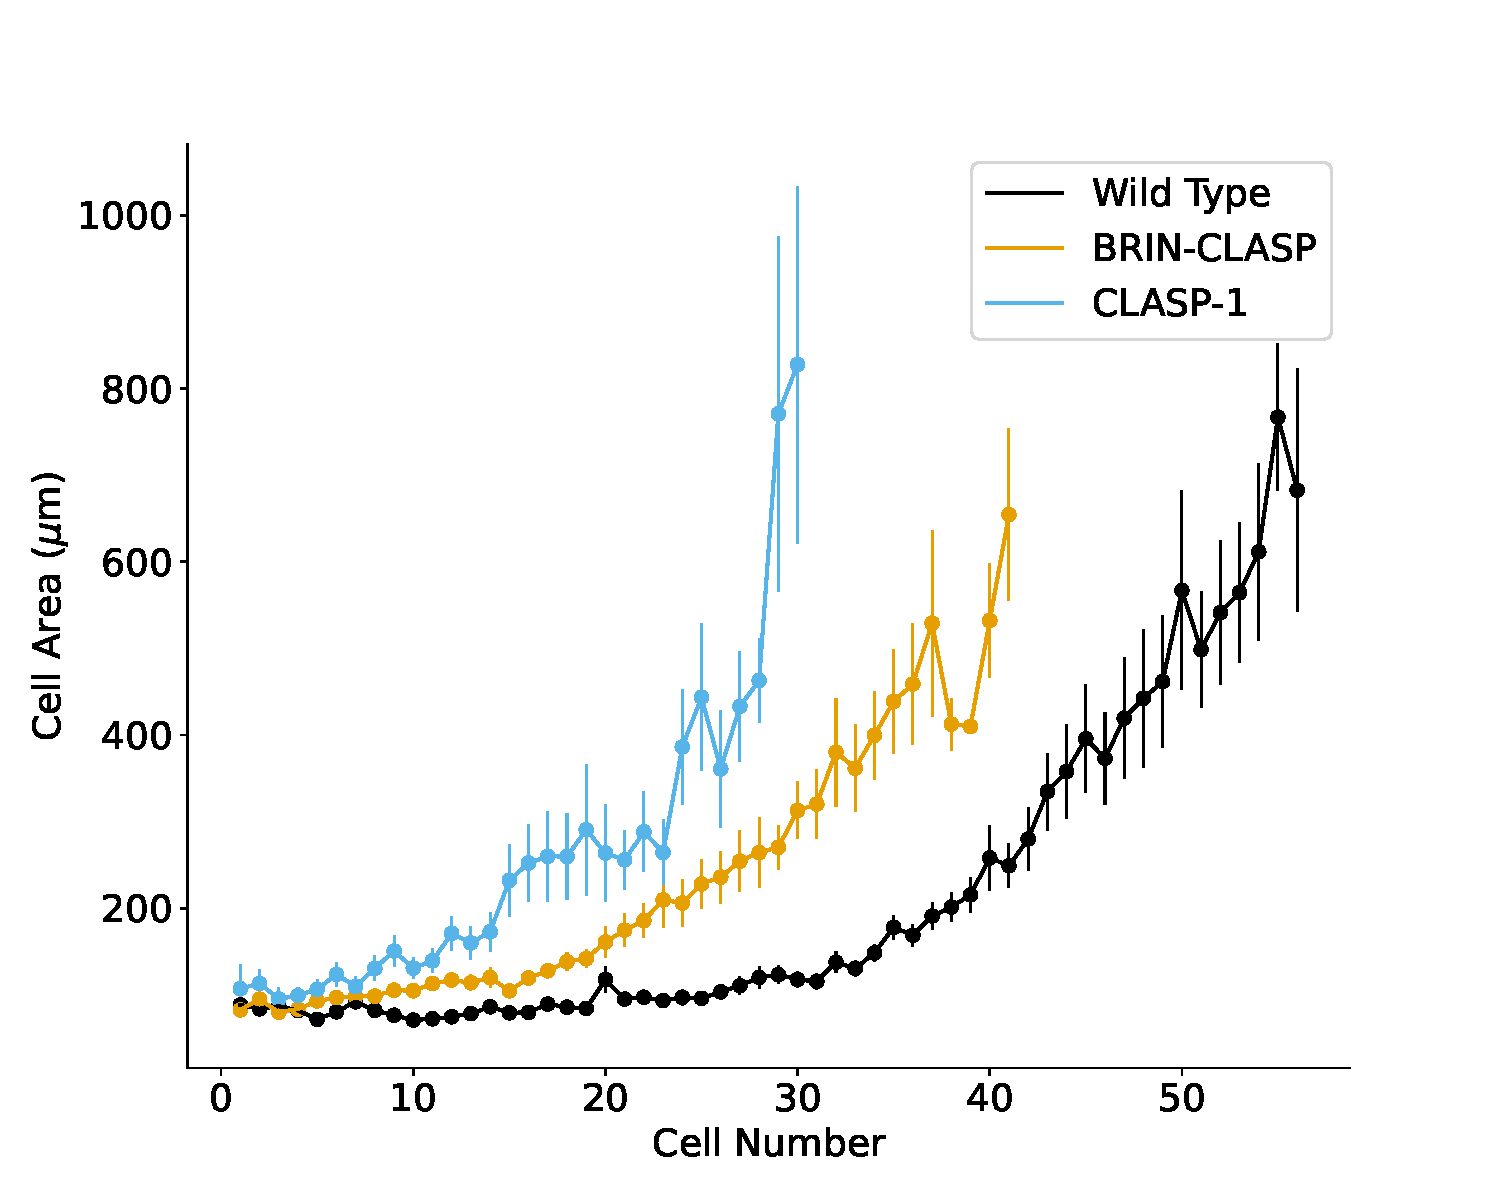
\includegraphics[width=\textwidth]{data-unprocessed.pdf}
  \caption{Raw data from the five distinct lines of \emph{A. thaliana} grown for this paper. The "Wild Type" data shown in black comes from both the \emph{Wild Type} and \emph{CLASPpro:GFP-CLASP/clasp-1} lines. The "BRIN-CLASP" data shown in orange comes from the \emph{brinCLASPpro:GFP-CLASP/clasp-1} lines (3) and (15). The "CLASP-1" data comes entirely from the \emph{clasp-1} lines. Differences in cell area between the mutants exhibit clear statistical significance. }
  \label{data-unprocesed}
\end{figure}

The raw data in units of cell number and cell area were transformed into units of cell position and cell length via the following procedure. First, the vertical cell faces were assumed to be flat so that the cross-sectional areas observed in the microscopy images correspond exactly to the length of the cell multiplied by its radius. Then, the position of each cell was determined by taking the cumulative sum of the lengths of the cells underneath it. By convention, cell position is relative to the quiescent centre, thus proximal cells are located higher. Missing data in the division zone was imputed using the average cell length by cell number. The resulting dataset contained position-length pairs from $0\um$ to $1500\um$ above the quiescent centre. However, the data above $500\um$ was omitted from subsequent analyses since it was noisy and sparse. 

\begin{figure}
  \centering
  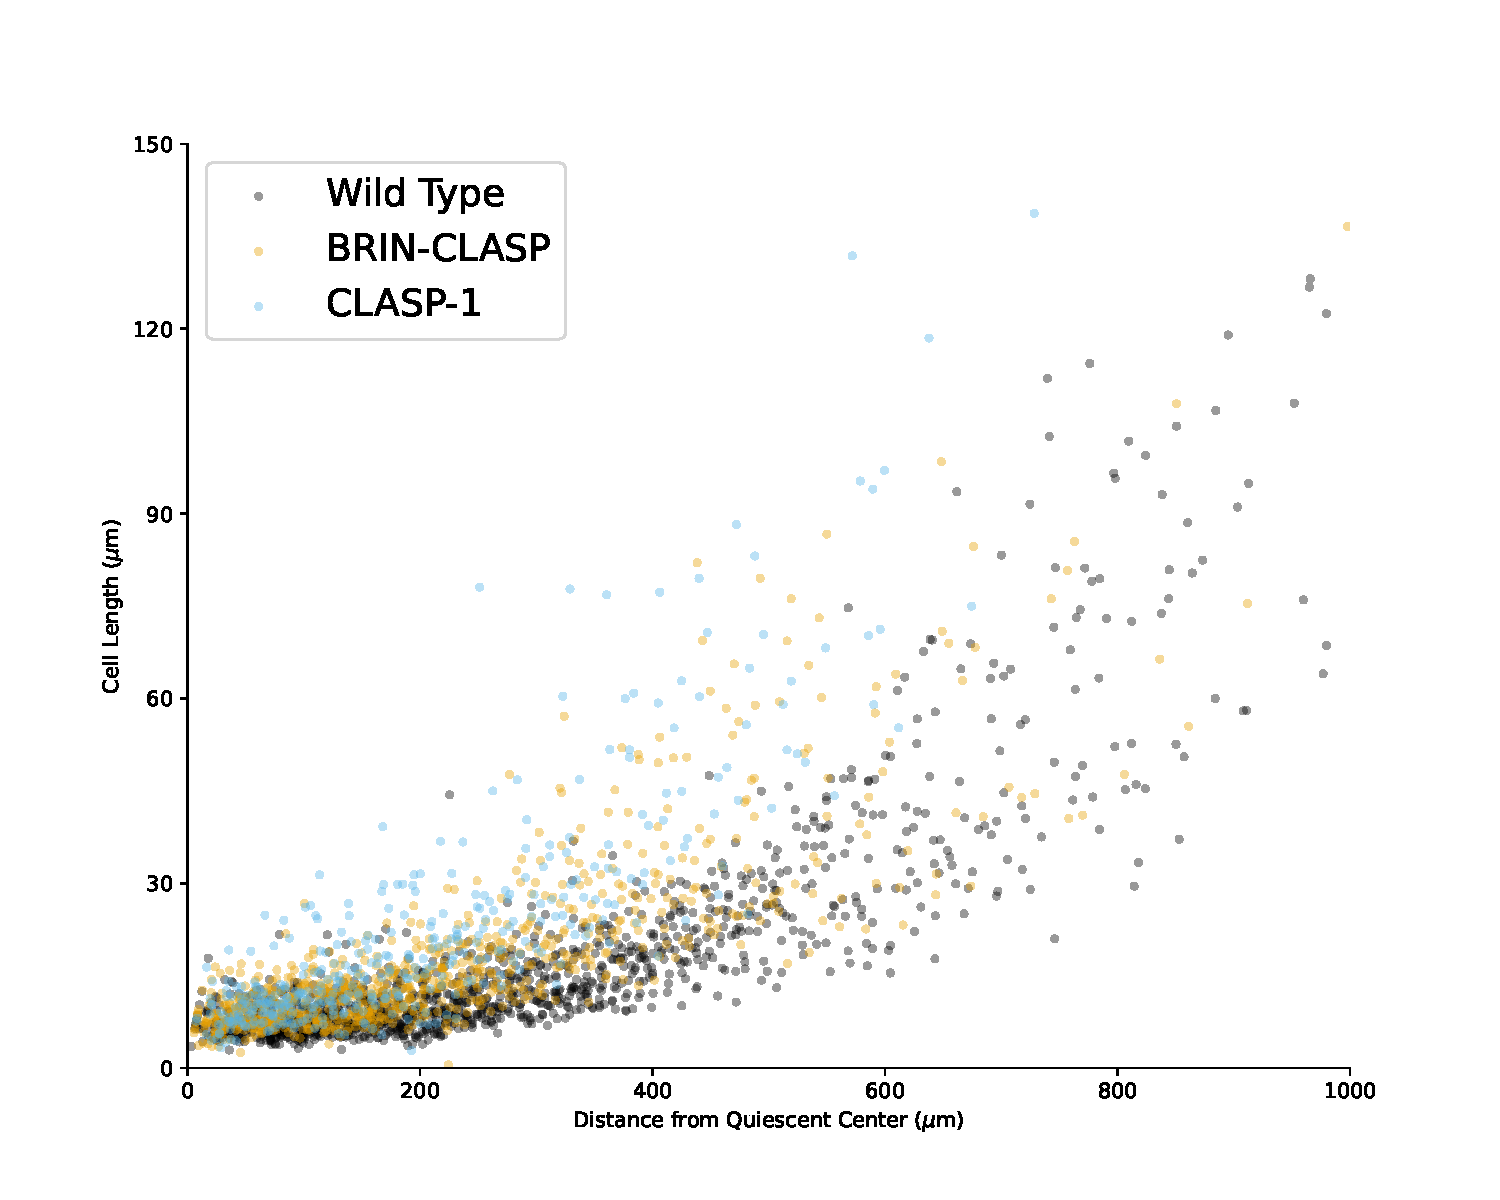
\includegraphics[width=\textwidth]{data-trichoblast.pdf}
  \caption{Raw data collected from trichoblast cells in \emph{A. thaliana}. There is a high density of data points in the distal region of the meristem ($< 500\um$), but significantly fewer data points between $500\um$ and $1000\um$, especially in the \emph{brinCLASPpro} and \emph{clasp-1} mutants. After binning this data (not shown) and computing the standard errors, we found that the data above $500\um$ was too noisy to differentiate the wild type and \emph{brinCLASPpro} mutant. }
  \label{data}
\end{figure}

\section{Model Derivation}\label{secA2}

Using the $R_{B}$ function shown in Equation \eqref{bri1} we can derive a mathematical description of the intracellular dynamics of the BR/CLASP signalling network over time using the system of ordinary differential equations shown in \eqref{intracellular-ode}. The parameters $s_{0}$, $c_{0}$, and $r_{0}$ represent basal production rates for BES1, CLASP, and BRI1 respectively. The parameters $s_{1}$, $c_{2}$, and $r_{2}$ represent decay rates for the same molecules. The parameter $c_{1}$ represents the rate at which the BES1 transcription factor inhibits the CLASP promoter while $r_{1}$ represents the rate at which CLASP promotes the recycling of endocytosed BRI1 receptors.

\begin{equation}
\label{intracellular-ode}
\begin{aligned}
  \frac{ d\text{BES1} }{ dt } &= s_{0}R_{B} - s_{1} \text{BES1} \\[5pt]
  \frac{ dC }{ dt } &= (c_{0} - c_{1}\text{BES1}) - c_{2}C \\[5pt]
  \frac{ dR_{T} }{ dt } &= (r_{0}  + r_{1}C) - r_{2}R_{T}
\end{aligned}
\end{equation}
Next, we assume that intracellular levels of BES1, CLASP, and BRI1 are in quasi-steady state (QSS), which means that $\frac{d\text{BES1}}{dt} = \frac{dC}{dt} = \frac{dR_{T}}{dt} = 0$. Using the QSS assumption gives us explicit formulas for $\text{BES1}$, $C$, and $R_{T}$ in terms of $R_{B}$ and each other, shown in Equation \eqref{intracellular-qss}. 

\begin{equation}
\label{intracellular-qss}
\begin{aligned}
  \text{BES1} &= \frac{ s_{0} R_{B}}{ s_{1} } \\[5pt]
  C &= \frac{ c_{0} - c_{1}\text{BES1} }{ c_{2} } \\[5pt]
  R_{T} &=\frac{ r_{0} + r_{1}C }{r_{2} } 
\end{aligned}
\end{equation}

Since $\text{BES1}$ is just a scalar multiple of $R_{B}$ we will use $R_{B}$ in place of $\text{BES1}$. It is known from \emph{in-vivo} experiments \cite{ruan2018} that the CLASP1 mutant had $65\%$ of the BRI1 receptors relative to the wild type. Since the wild type root has a BRI1 receptor concentration of approximately $62\text{nmol L}^{ -1 }$ \cite{vanesse2012}, this tells us that the \emph{clasp-1} mutant should have a BRI1 receptor concentration of approximately $(62 \cdot 0.65)\text{nmol L}^{ -1 }$. If we let $C = 1$ denote the average concentration of the CLASP protein in the wild type and recall that the \emph{clasp-1} mutant should satisfy $C = 0$, we can define a simplified equation \eqref{clasp-simplified} governing the CLASP protein.

\begin{equation}
\label{clasp-simplified}
\left.\begin{aligned}
  62 = (r_{0} + r_{1}) / r_{2} \\
  62 \cdot 0.65 = r_{0} / r_{2}
\end{aligned}\right\rbrace \Rightarrow  \frac{r_{1}}{r_{2}} = 62 \cdot 0.35
\end{equation}

Finally, we define the new parameters $\beta_{0} = \frac{c_{0}}{c_{2}}$, $\beta_{1} = \frac{c_{1}}{c_{2}}$. This gives us two new equations \eqref{intracellular-final} for the intracellular protein concentrations of CLASP and BRI1 under the QSS assumption.

The intracellular dynamics influence the rates of cell division and elongation. We can add this to our model by including the two additional ODEs in Equation \eqref{extracellular-ode}. In these equations, BES1 promotes cell growth at a rate $\gamma_{1}$. The rate of cell elongation is assumed to be proportional to length because longer cells have more vertical surface area for the cellulose microfibrils to stretch. This modelling assumption is also known from the literature \cite{lockhart1965, smithers2024}. The variable $D \in [0, 1]$ denotes the cell's position in the cell cycle. When $D = 1$, the cell divides into two cells of equal length with $D = 0$. Progress in the cell cycle proceeds at a basal rate $d_{0}$, which is augmented by CLASP at a rate $d_{1}$. As cells grow past a critical length $d_{2}$, they stop progressing through the cell cycle entirely. 

\begin{equation}
\label{extracellular-ode}
\begin{aligned}
  \frac{ dL }{ dt } &= \left(\gamma_{0} + \gamma_{1}\text{BES1}\right)L  \\[5pt]
\frac{ dD }{ dt } &= (d_{0} + d_{1}C)\left( 1 - \frac{ L^{ n } }{ d_{2}^{ n } + L^{ n } } \right) 
\end{aligned}
\end{equation}

The ODE model presented in \ref{22} has over fifteen parameters, which would result in a redundant and overfitted model if used directly on the experimental data. To simplify the model, we make several assumptions. First, we fix $d_{0} = 1$ since our data and thus our model has no time-dependence. Therefore, time is a dimensionless variable that we can rescale as needed. Defining $\delta_{0} = \frac{d_{1}}{d_{0}}$ and $\delta_{1} = d_{2}$ gives us the dimensionless equation for $D$ shown in Equation \eqref{extracellular-final}.

\section{Additional Figures}\label{secA3}

\begin{figure}
  \centering
  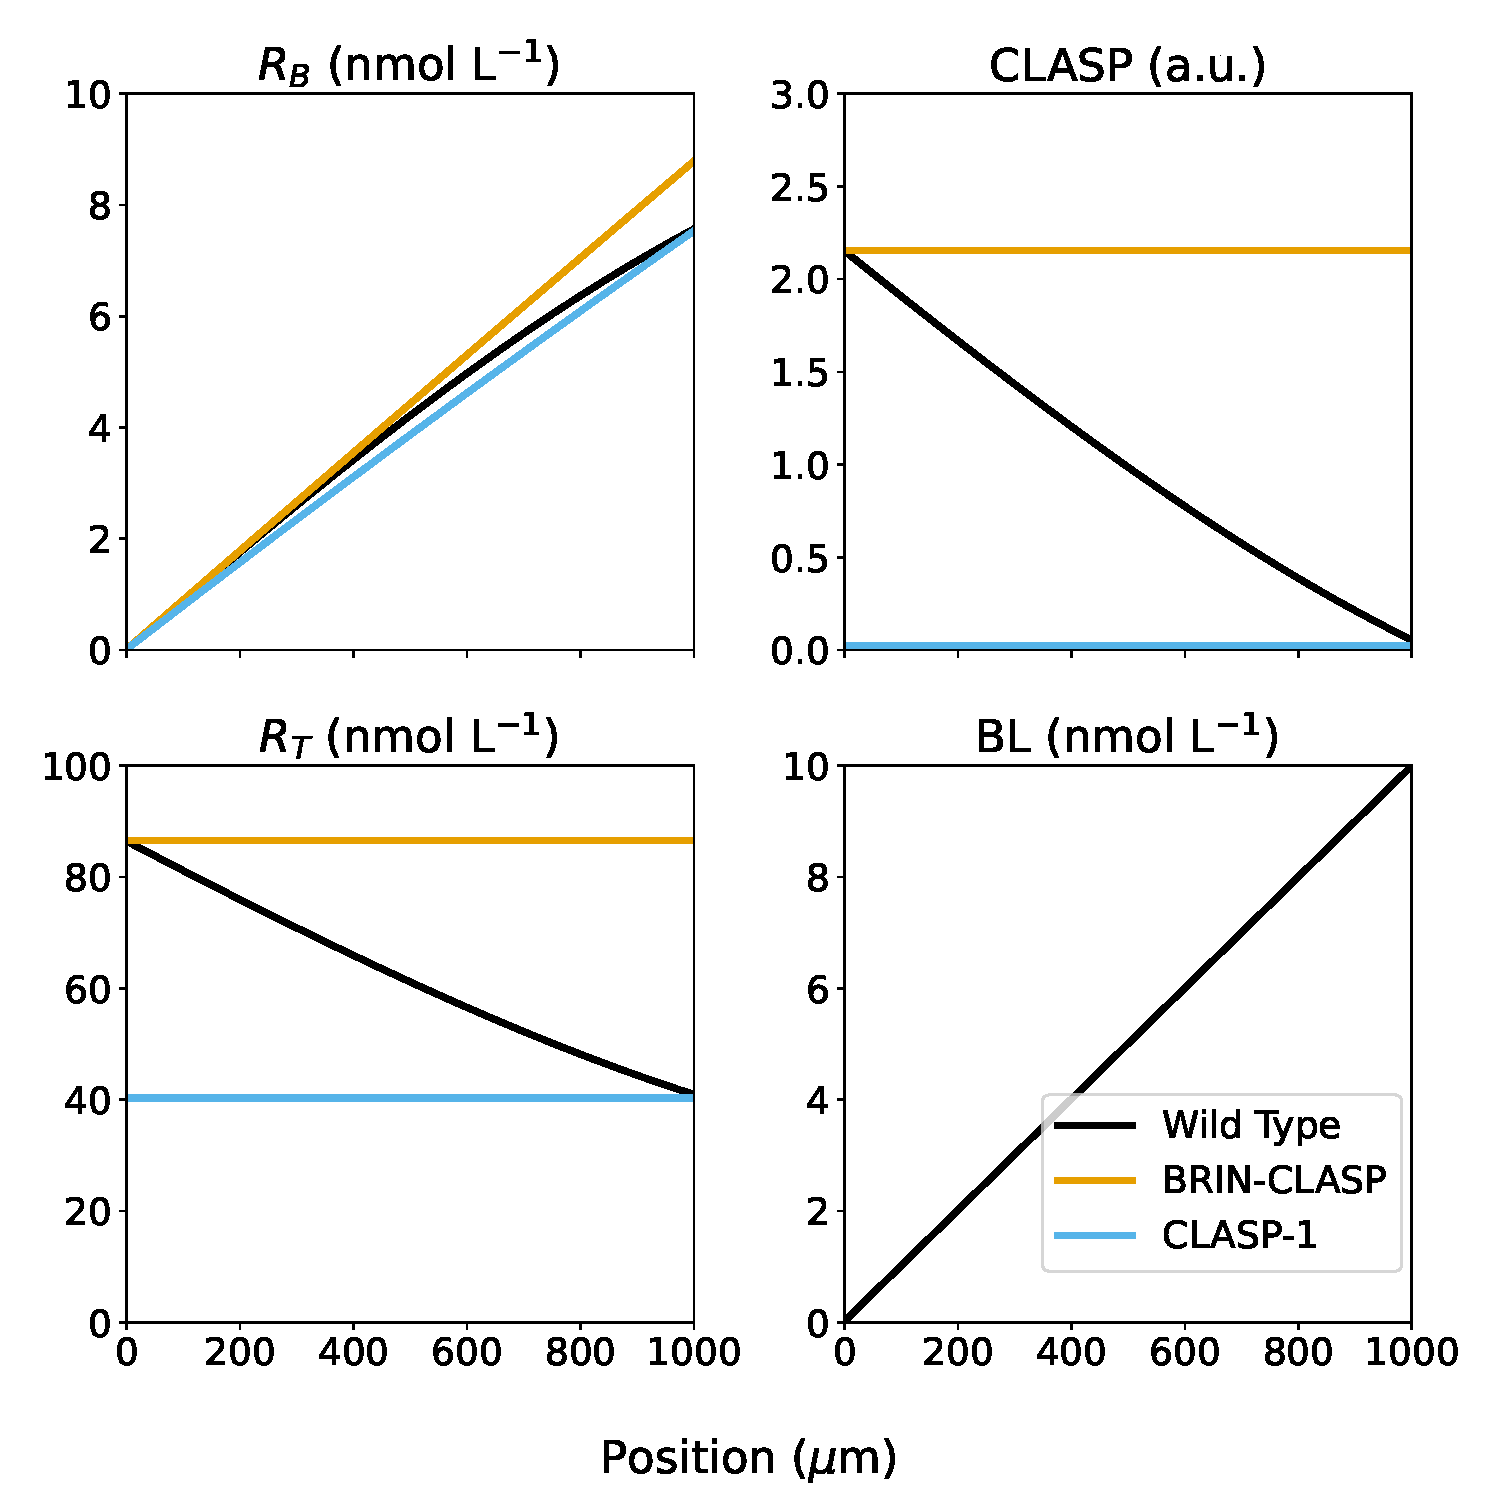
\includegraphics[width=\textwidth]{bes1-mutants-modified.pdf}
  \caption{Results of modifying the intracellular system to increase the rate of cell elongation in the \emph{brinCLASPpro} mutant. The plot shown has a value of $B^{*} = \omega B$ where $\omega = 10$. This means that we are assuming that brassinosteroids other than BL have $10$ times the effect of BL on BES1 signalling. Even with such a large choice of $\omega$, the model cannot differentiate the bound BRI1 concentration $R_{B}$ in the \emph{brinCLASPpro} mutant from the wild type.}
  \label{bes1-mutants-modified}
\end{figure}

\begin{figure}
  \centering
  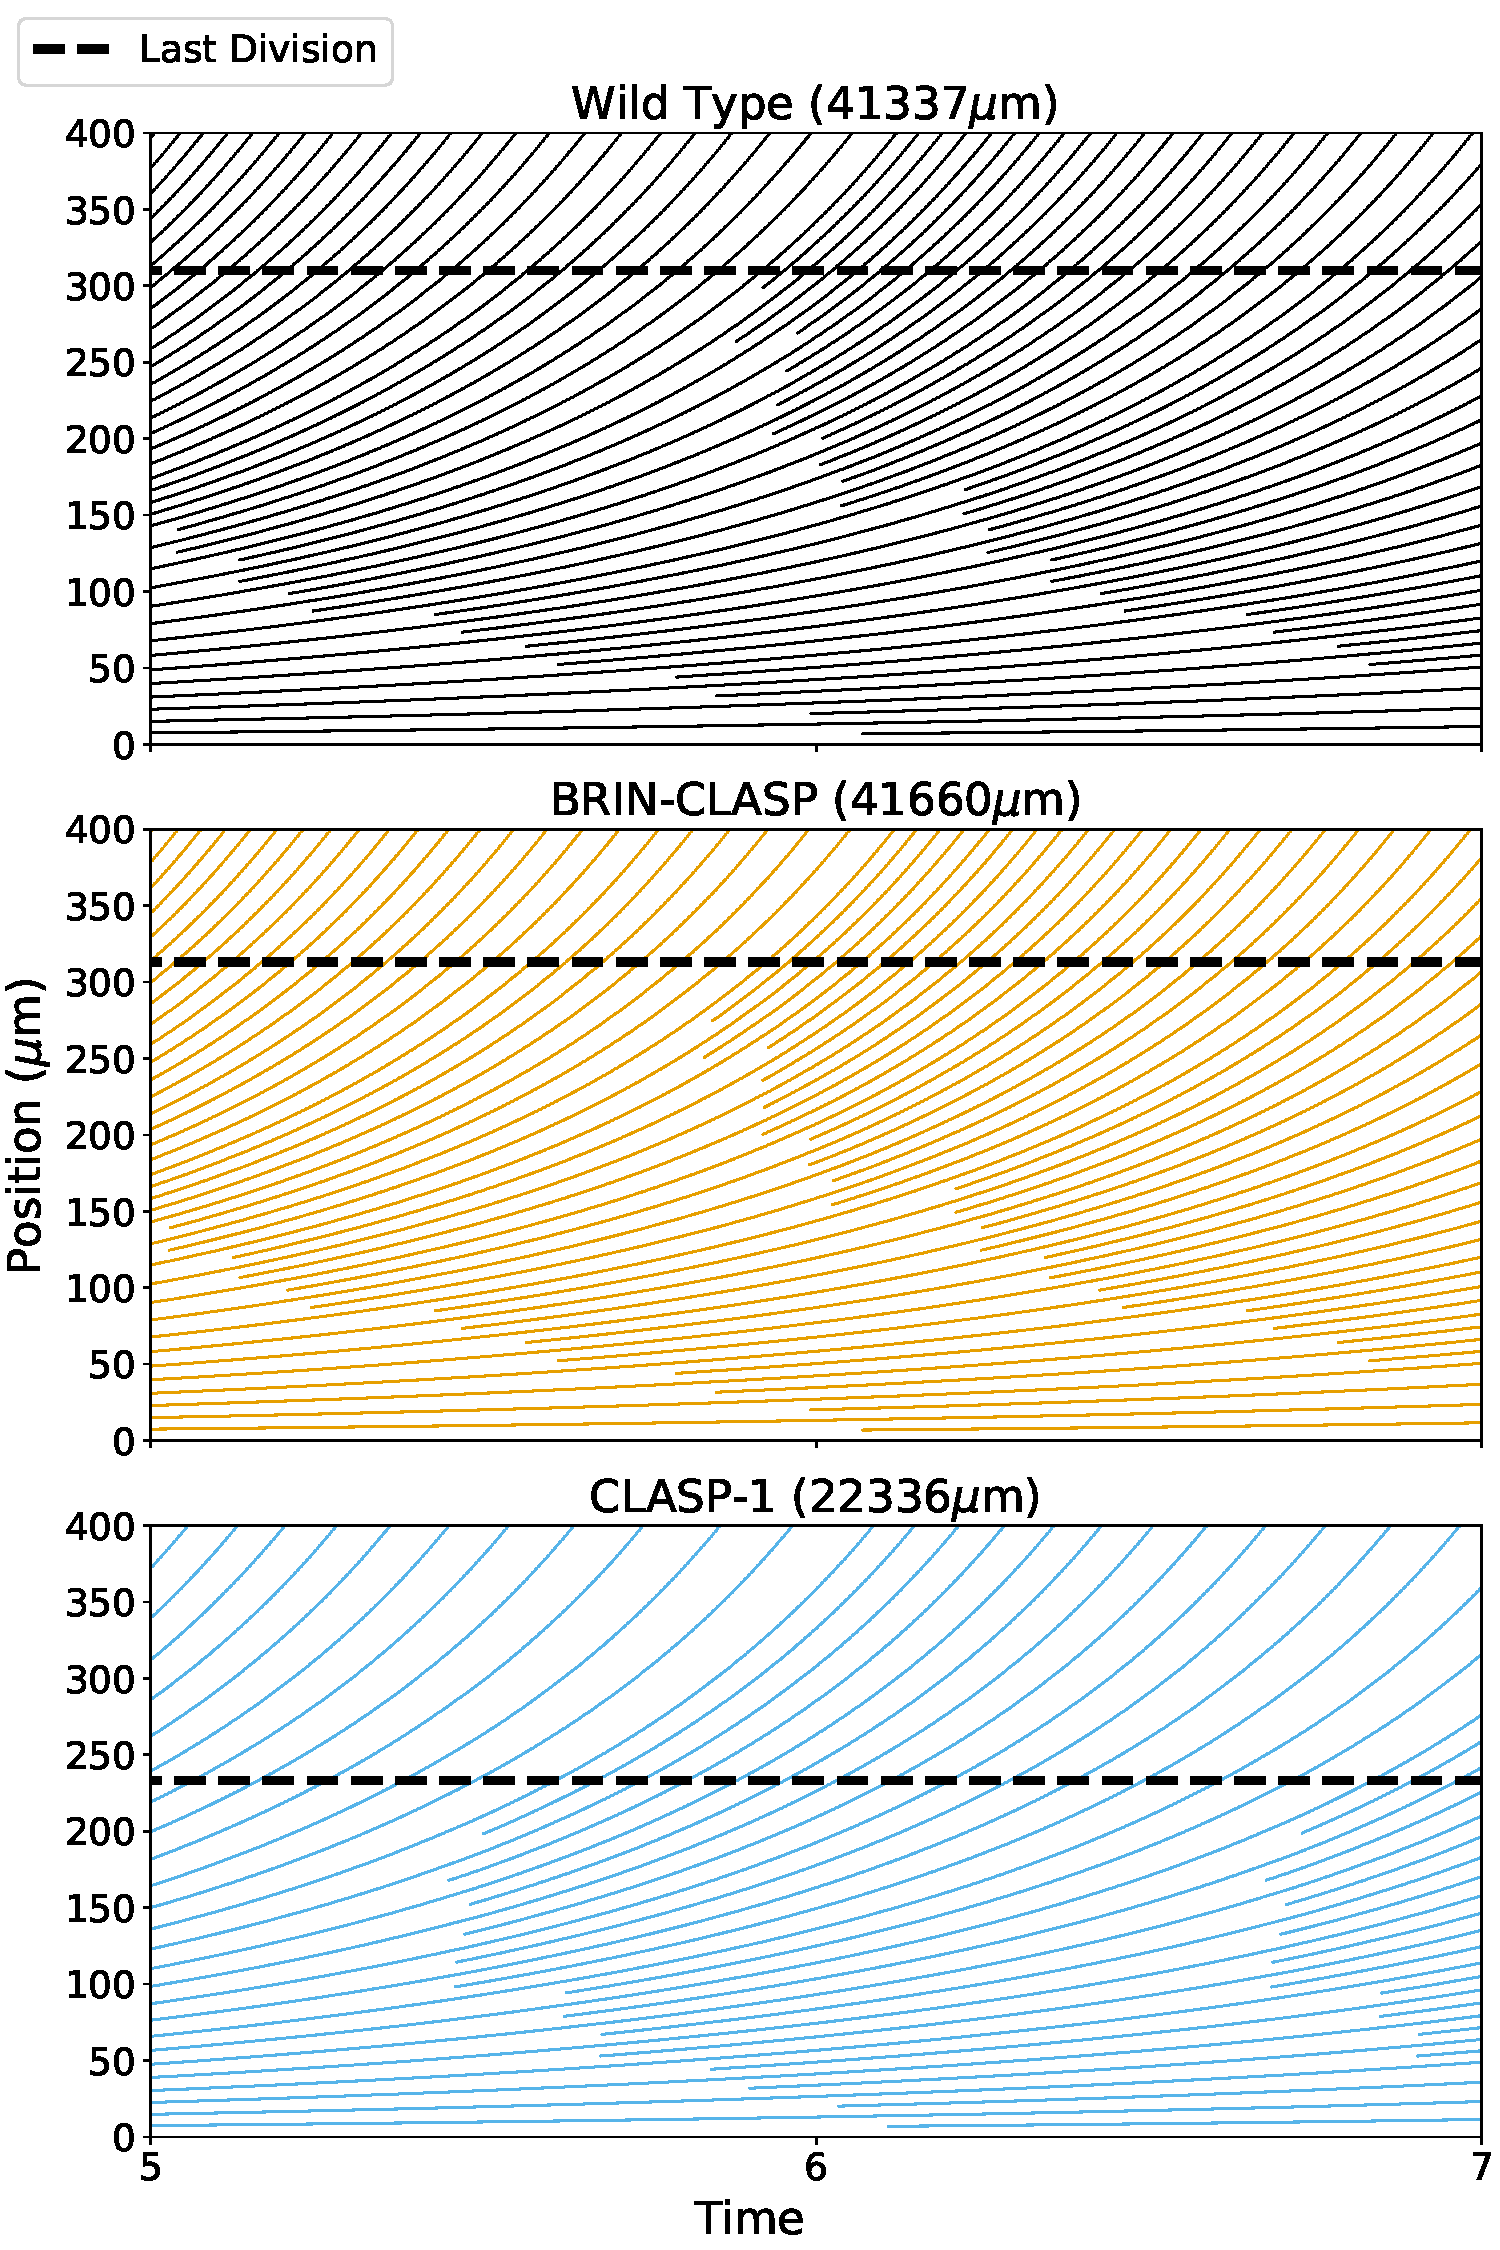
\includegraphics[height=500pt]{column-original-profile.pdf}
  \caption{Cell column projection for the original column model.}
\end{figure}

\begin{figure}
  \centering
  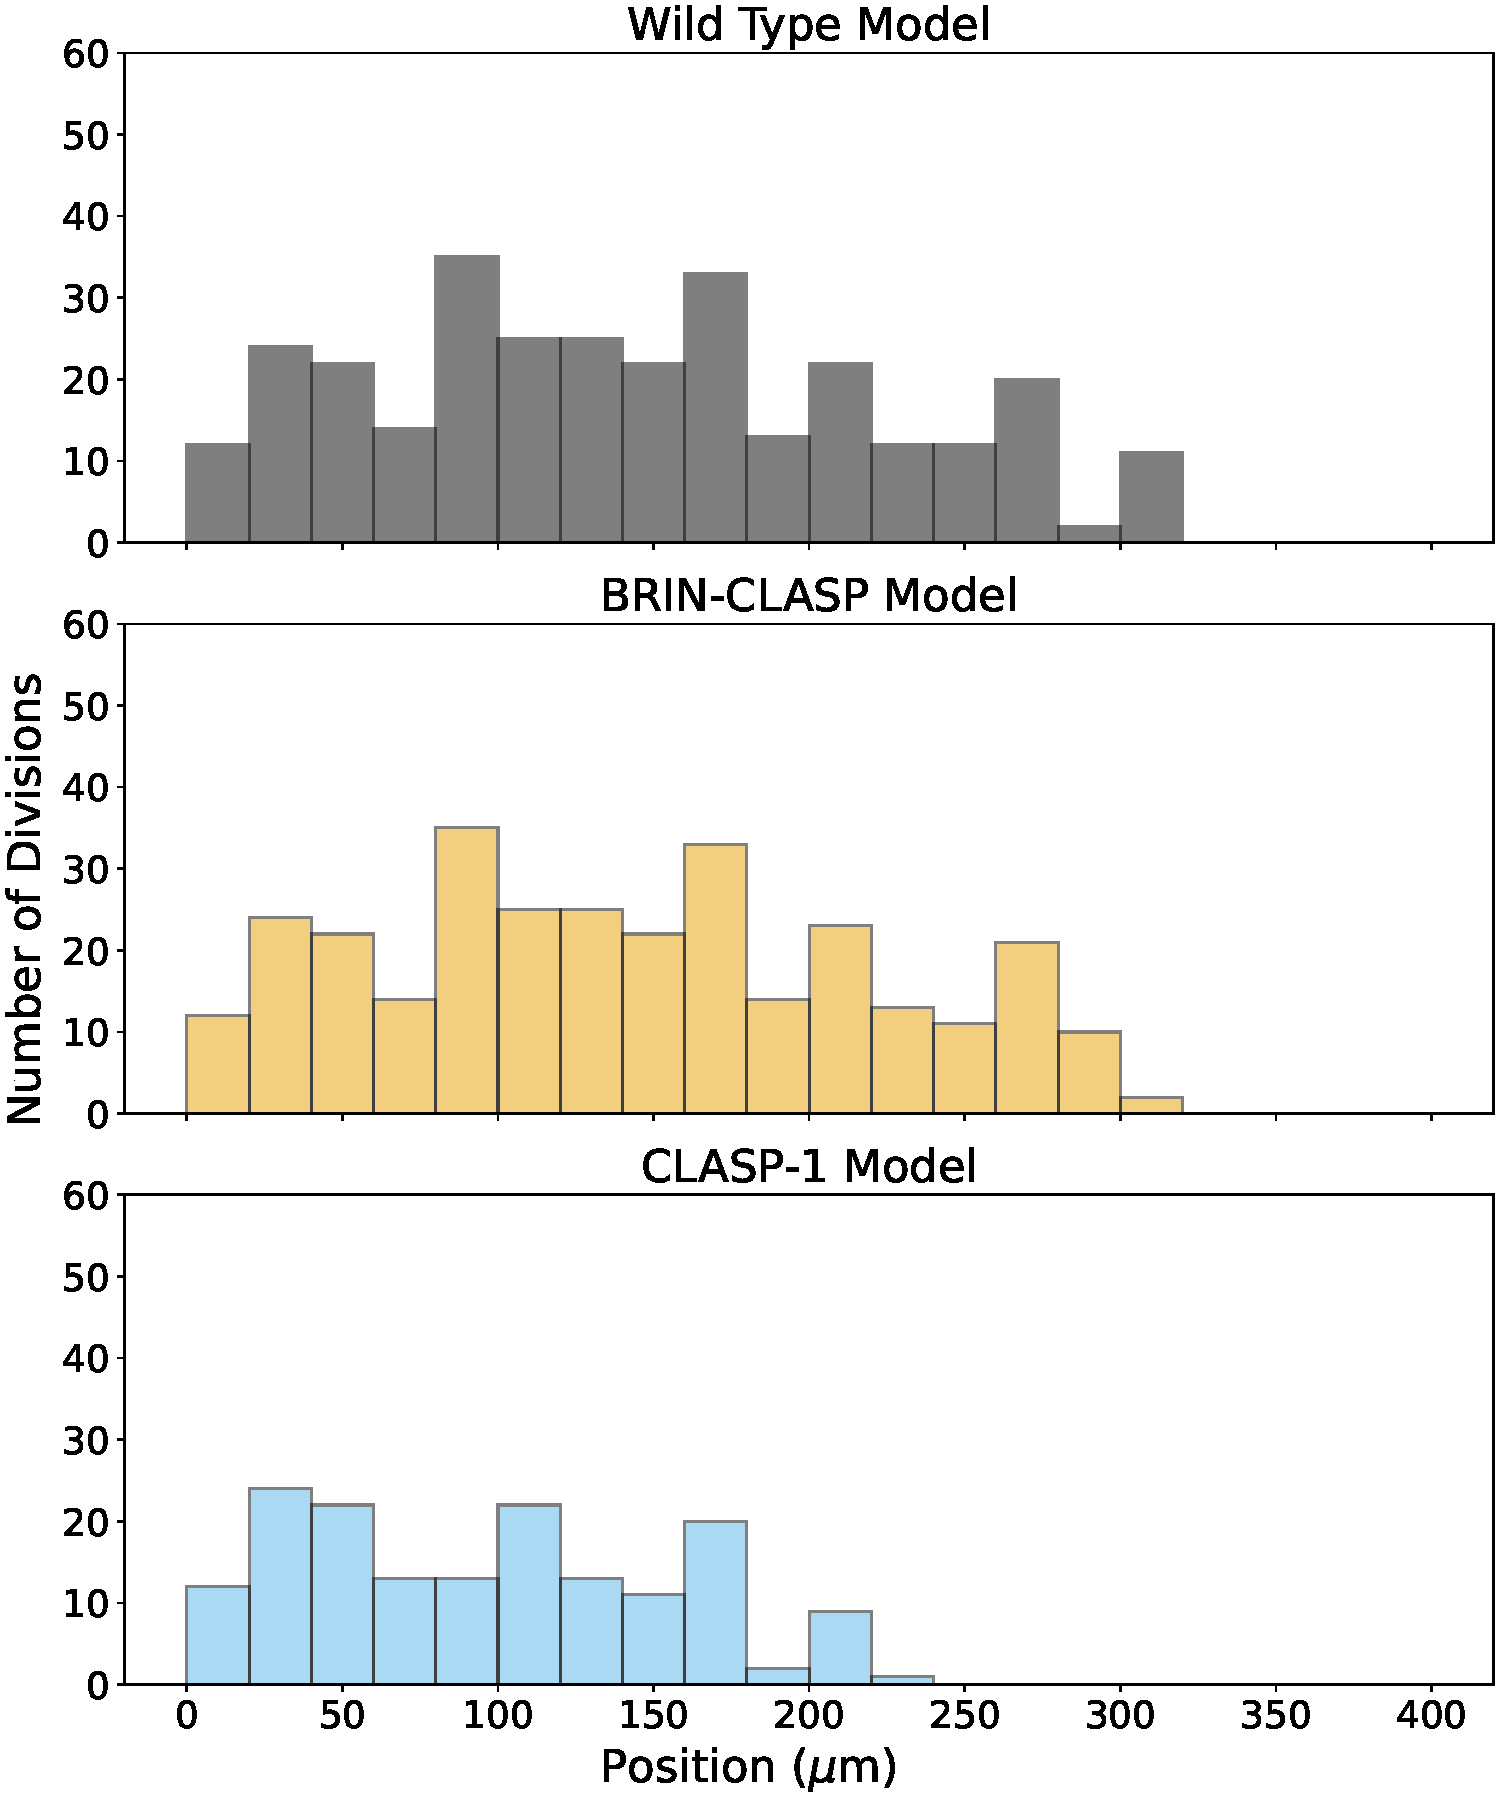
\includegraphics[width=\textwidth]{column-original-histogram.pdf}
  \caption{Histogram of division locations for the original column model.}
\end{figure}

\begin{figure}
  \centering
  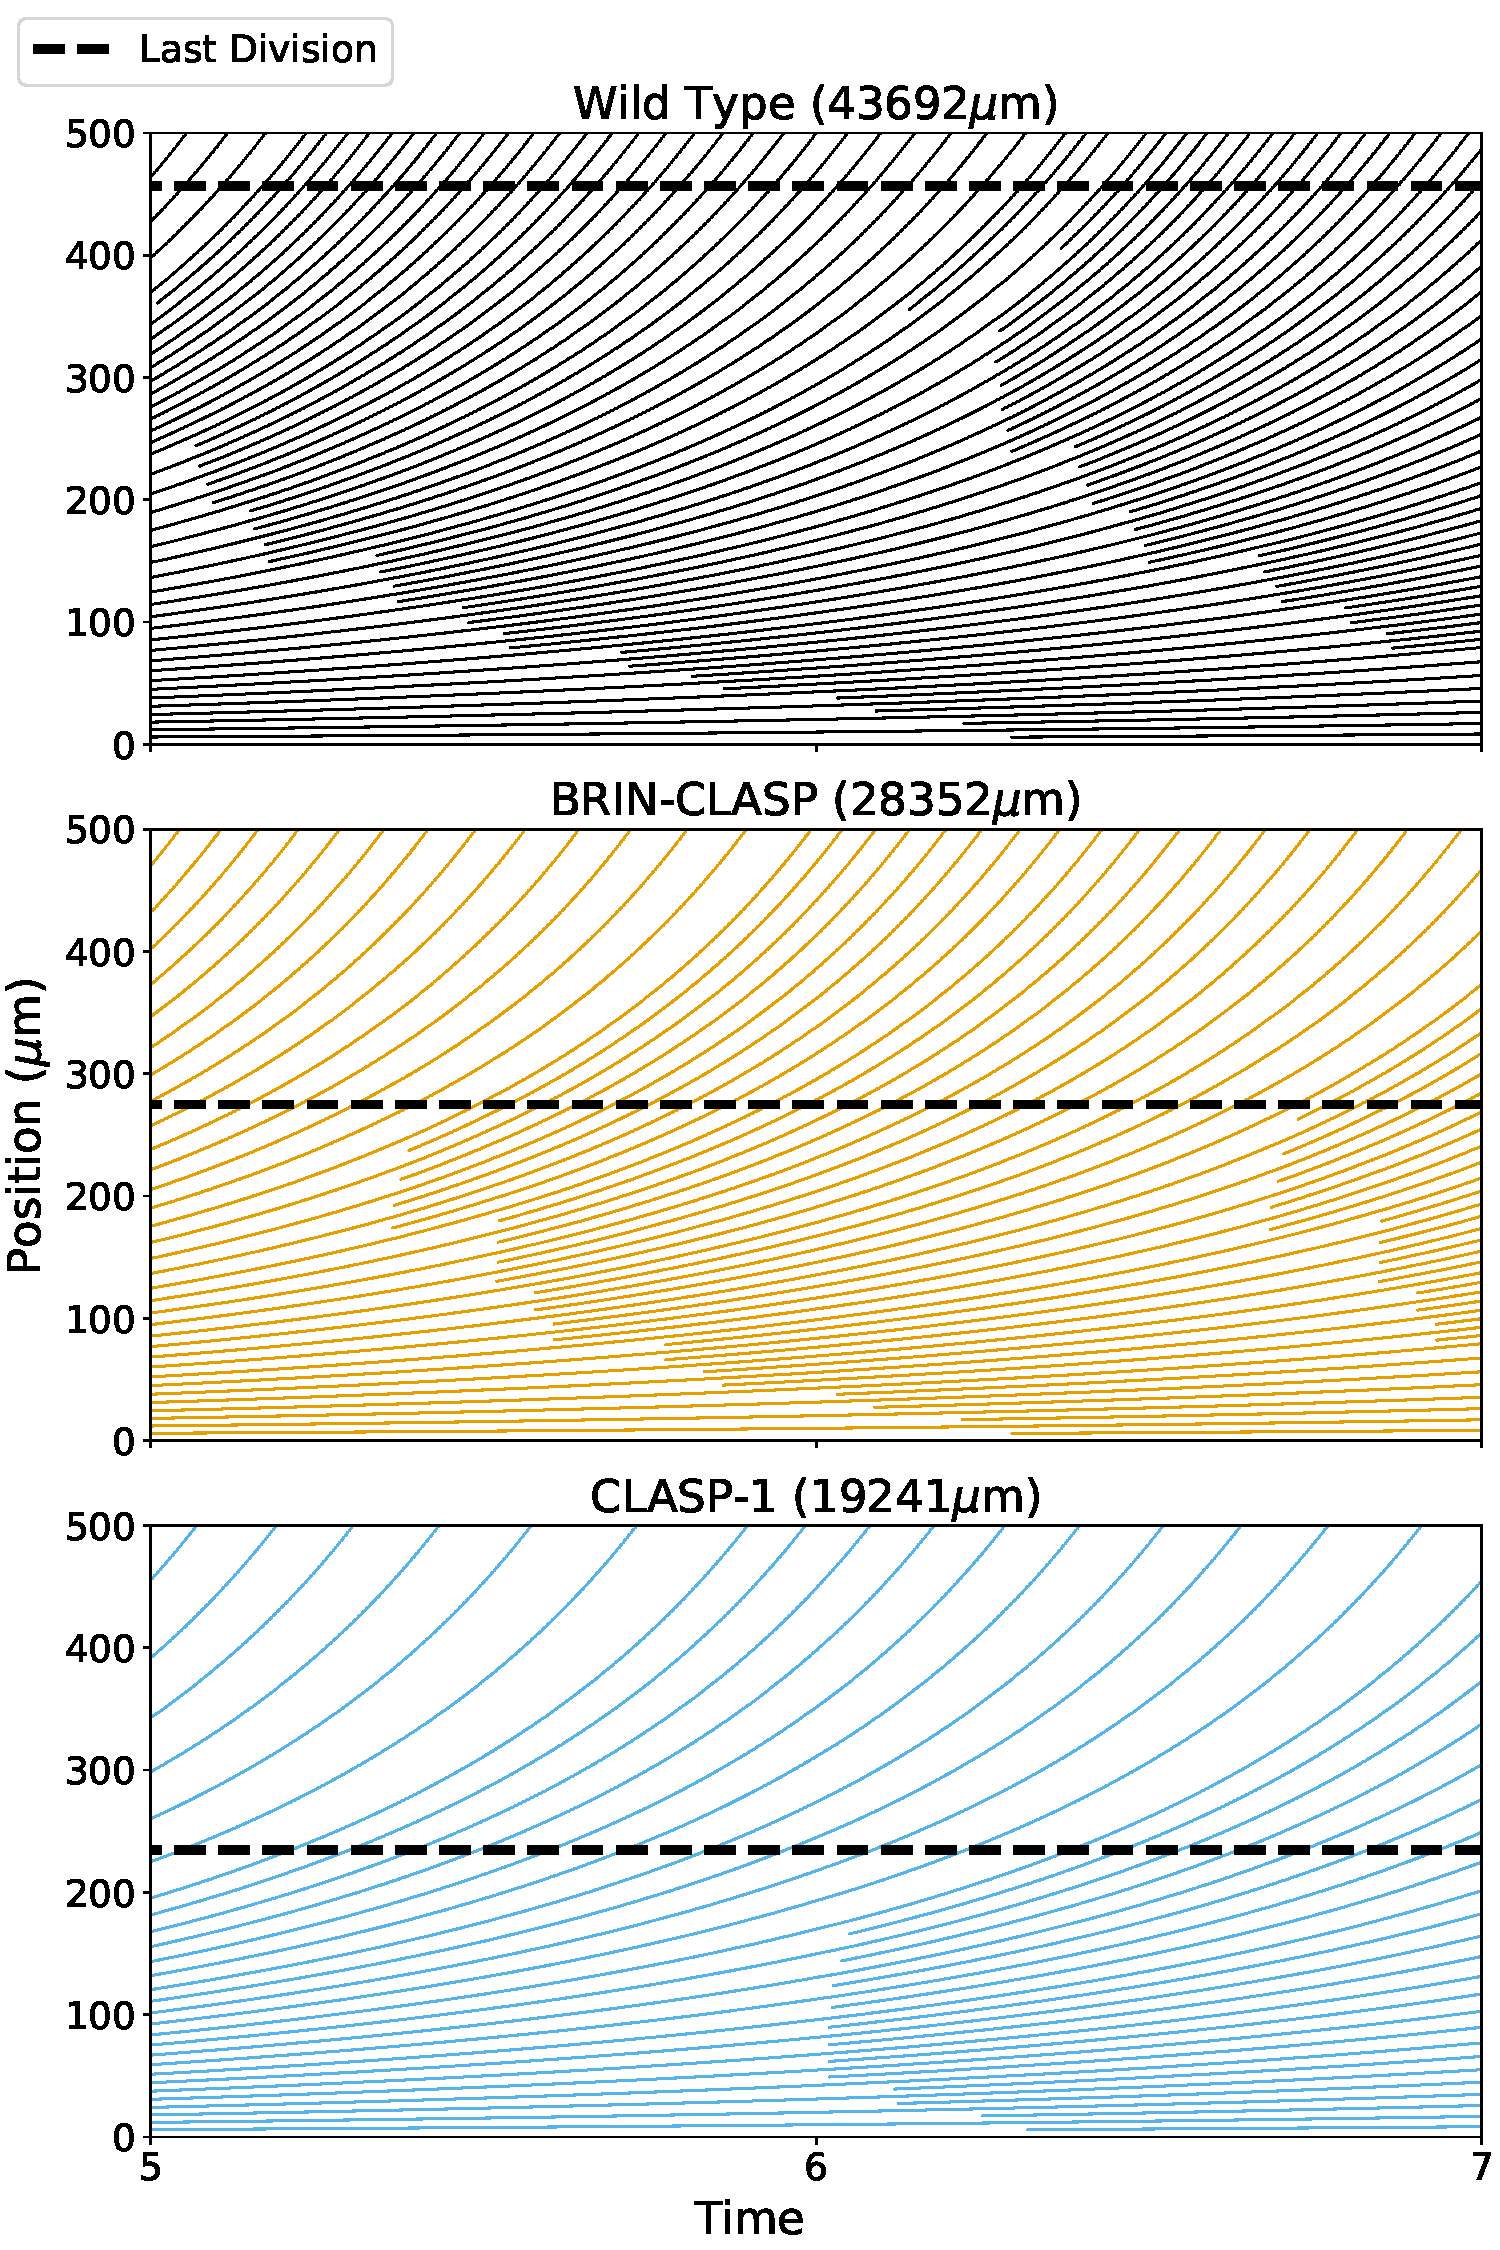
\includegraphics[height=500pt]{column-modified-profile.pdf}
  \caption{Cell column projection for the modified column model.}
\end{figure}

\begin{figure}
  \centering
  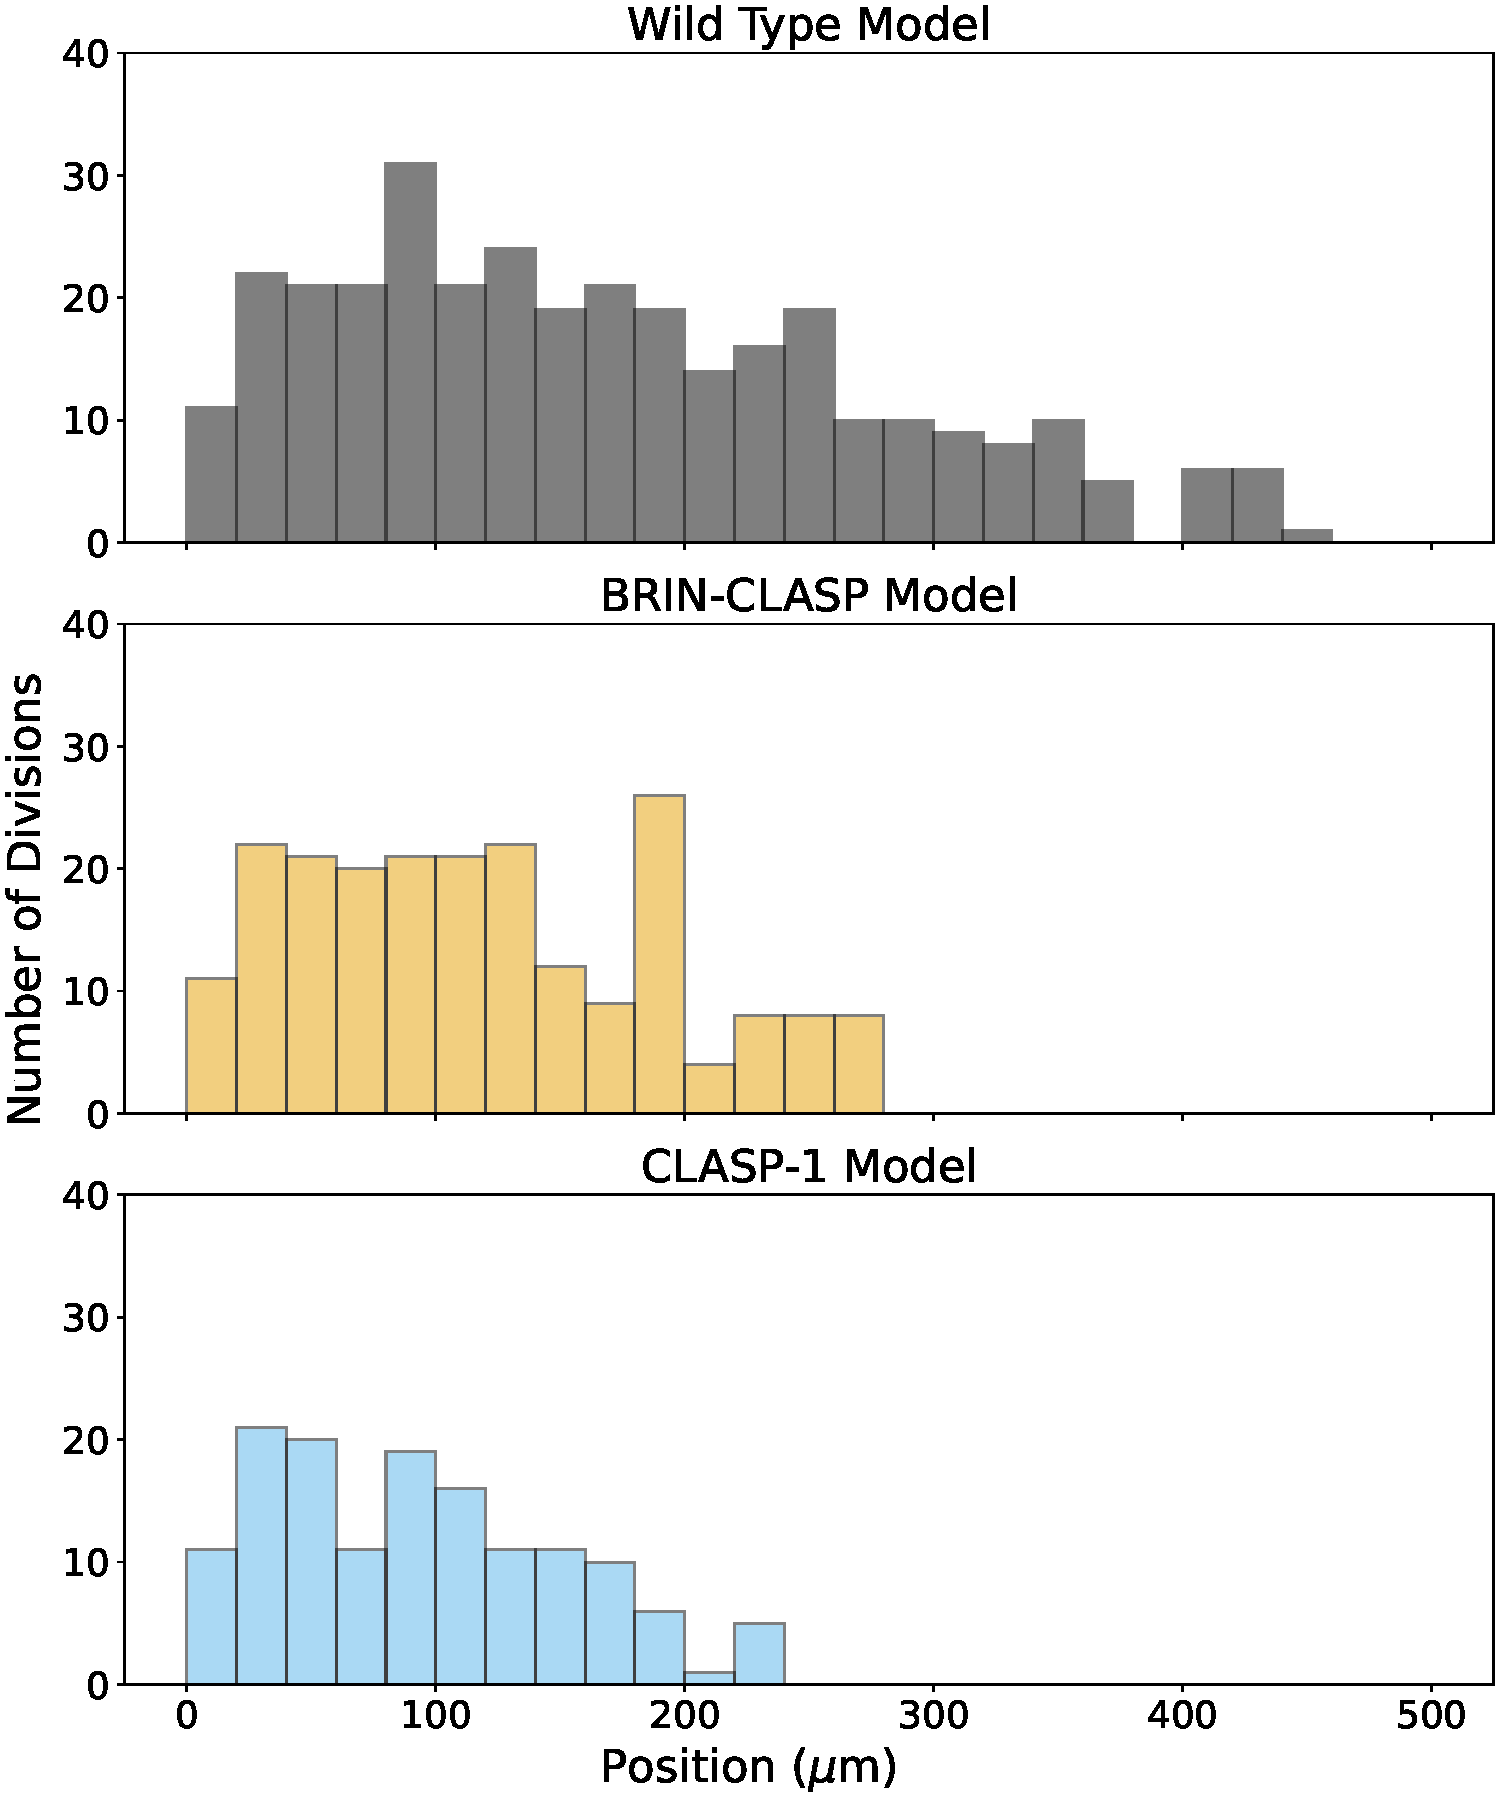
\includegraphics[width=\textwidth]{column-modified-histogram.pdf}
  \caption{Histogram of division locations for the revised column model.}
\end{figure}

\section{Atrichoblast Model}\label{secA4}

The data used in this project was collected from trichoblast and atrichoblast cells from the epidermal cell columns of \emph{A. thaliana} roots. In this appendix, we compare qualitative observations from the trichoblast and atrichoblast cell columns and contrast the fitted models for both of these datasets. Figure \ref{column-atrichoblast-fit} presents the fitted mode for atrichoblast cells, while Table \ref{column-atrichoblast-parameters} compares parameter values for the trichoblast and atrichoblast column models.

\begin{figure}
  \centering
  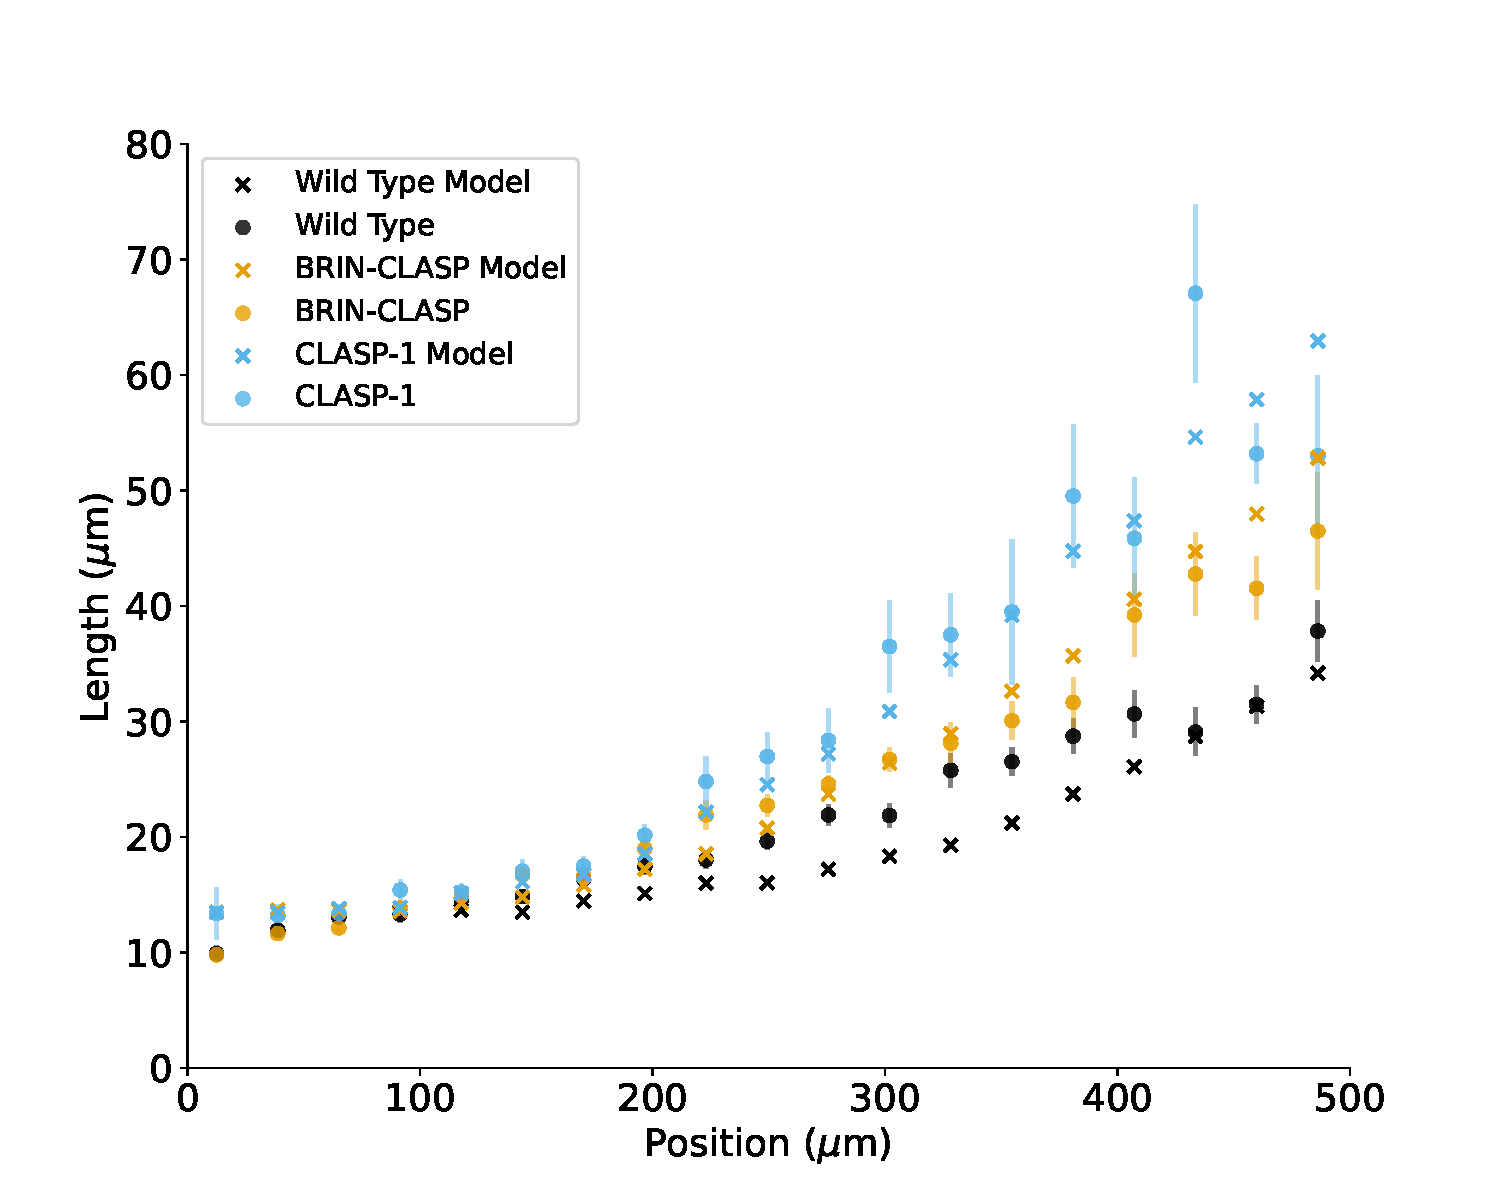
\includegraphics[width=\textwidth]{column-atrichoblast-fit.pdf}
  \caption{Results of fitting the model to atrichoblast data. The model has some inaccuracies at lower positions but accurately captures the trend of the data. Compared to trichoblast cells, atrichoblast cells exhibit less differentiation between the mutants and have longer cells on average. }
  \label{column-atrichoblast-fit}
\end{figure}

\begin{table}[!ht]
\centering
\label{column-atrichoblast-parameters}
\begin{tabular}{@{}lllllllll@{}}
\toprule
Model & RMSE & $m$ & $\gamma_{0}$ & $\gamma_{1}$ & $\delta_{1}$ & $\sigma_{0}$ & $\sigma_{1}$ \\
\midrule
Trichoblast & $4.648$ & $11.69$ & $0.4877$ & $4.165$ & $23.44$ & $0.8333$ & $1.463$ \\
Atrichoblast & $10.895$ & $14.23$ & $0.4630$ & $5.086$ & $28.86$ & $0.8333$ & $1.488$ \\
\botrule
\caption{Optimal parameter values for the atrichoblast column model compared to the trichoblast column model. Both models use the biphasic CLASP function described in the paper. The atrichoblast model has higher $m$ and $\delta_{1}$ parameters, which makes sense because atrichoblast cells are larger. Other parameters remained roughly the same, which suggests that the estimated parameters are relatively robust to changes in the data.} 

\end{tabular}
\end{table}

\end{appendices}

\end{document}
